\documentclass[12pt]{report}

%%%%%%%%%%%%%%%%%%%%%%%%%%%%%%%%%%%%%%%%%%%%%%%%%%%%%%%%%%%%%%%%%%%%%%%%
\usepackage{pdfsync}        % allows clicking in PDF to take you back to the text

\usepackage{lmodern}        % use modern latin fonts
% \usepackage{palatino}        % use modern latin fonts
% \usepackage{times}        % use modern latin fonts
\usepackage[T1]{fontenc}    % use 8 bit output font encoding with more glyphs
\usepackage[utf8]{inputenc} % so you can type ă
% \usepackage{siunitx}        % automatically formats numbers with spaces and all that

\usepackage[dvipsnames]{xcolor}         % more color choices
\usepackage[english=british]{csquotes} % for correct use of `` '' ... TODO!!
\usepackage{url}            % typeset URL's sensibly
\usepackage[nottoc]{tocbibind} % include bibliography in ToC (third-rep.cls not working)
\usepackage{appendix} % customise the appearance of appendix via an 'appendix' environment

% \usepackage{tabu}
\usepackage{array}
\usepackage{colortbl}
\usepackage{colortbl}
\definecolor{LightGreen}{HTML}{9bffa0}

\usepackage{layouts} % allows you to print lengths

% set line space nicely (only for text, not captions etc)
\usepackage{setspace}
\onehalfspacing

\usepackage[a4paper,textwidth=159mm, hmargin ratio=1:1, vmargin ratio=1:1, verbose]{geometry}
\makeatletter
\AtEndPreamble{%
  \normalfont
  \ifcase \@ptsize
    \geometry{textheight=240mm}%
    \or
    \geometry{textheight=243mm}%
    \or
    \geometry{textheight=241mm}%
  \fi
}

\usepackage{enumitem} % configure labels of items in enumerations i.e. i), ii)
\setlist[description]{style=nextline,font=\normalfont\textbullet\space,labelindent=\parindent}


\usepackage{natbib}
\setcitestyle{authoryear,round}

% the starred \newcommand is more strick wrt the arguments it takes (cannot contain paragraph)
% so \newcommand* should be the default you use
\definecolor{ToDoColor}{rgb}{0.4,0.4,0.4}
\newcommand{\todo}[1]{\textcolor{ToDoColor}{ToDo: #1}}
\newcommand*{\startToDo}{\color{ToDoColor}ToDo: \\}
\newcommand*{\stopToDo}{\color{Black}}

%% =============================================================================
% Remove "Chapter x" line before a new chapter
% This should be in .cls file, ideally
\makeatletter
\renewcommand{\@makechapterhead}[1]{%
  % \vspace*{15 pt}% Space before the chapter name
  {\setlength{\parindent}{0pt} \raggedright \normalfont
    \bfseries\Huge
    #1% The chapter's name
    \par\nobreak\vspace{35 pt}}} % Space after chapter name
\makeatother
%% =============================================================================

\usepackage{amsmath, amssymb,mathtools,bm}
\usepackage{bbm}
\DeclareMathOperator*{\argmin}{argmin} % * means the argument in _{} is placed below rather than to the right
\DeclareMathOperator{\argmax}{argmax} % * means the argument in _{} is placed below rather than to the right
\DeclareMathOperator{\iou}{IoU}
\DeclareMathOperator{\AP}{\operatorname{AP}_{\iou > 0.5}}
\DeclareMathOperator{\cer}{CER}
\DeclareMathOperator{\wer}{WER}
\providecommand{\CER}[1]{\( \operatorname{CER} = #1\% \)}
\providecommand{\WER}[1]{\( \operatorname{WER} = #1\% \)}
\providecommand{\norm}[1]{\lVert#1\rVert} % unlike \newcommand, this does nothing if \norm already exists
\providecommand{\card}[1]{\left\vert#1\right\vert}
% \DeclarePairedDelimiter\norm{\lVert}{\rVert}
% \DeclarePairedDelimiter\card{\left\vert}{\right\vert}
\DeclarePairedDelimiter\ceil{\lceil}{\rceil}
\DeclarePairedDelimiter\floor{\lfloor}{\rfloor}

\newcommand*{\ve}[1]{\mathbf{#1}} % for displaying a vector
\newcommand*{\ma}[1]{\mathrm{#1}} % for displaying a matrix
\newcommand*{\cls}{\mathit{cls}} % for RPN loss
\newcommand*{\reg}{\mathit{reg}}
% this makes the symbol := look nicer
\mathchardef\ordinarycolon\mathcode`\:
\mathcode`\:=\string"8000
\begingroup \catcode`\:=\active
  \gdef:{\mathrel{\mathop\ordinarycolon}}
\endgroup


%----------------------------------------------------------------------------------------
\usepackage{graphicx}
  \graphicspath{{./images/}}
  \setkeys{Gin}{width=\linewidth} % set \includegraphics default width
  \makeatletter
    \let\ginnatwidth\Gin@nat@width
    \let\ginnatheight\Gin@nat@height
  \makeatother
  \usepackage[export]{adjustbox} % used to align some images with the text between them (valign=c)
%----------------------------------------------------------------------------------------

\usepackage[compatibility=false]{caption}
\usepackage{subcaption}
\usepackage{floatrow}       % automatically centers floats
  % \subref -> '(a)' rather than just 'a'
  \captionsetup[subfigure]{subrefformat=simple,labelformat=simple}
  \renewcommand\thesubfigure{(\alph{subfigure})}
  \makeatletter
  \renewcommand\p@subfigure{\thefigure~}
  \makeatother
  % make the caption a bit shorter than the rest of the text, with bold font for label
  \captionsetup{margin=10pt,labelfont=bf,indention=.5cm}

  \newcommand{\rulesep}{\unskip\ \vrule\ } % allows to draw vertical line between figures
  % \makeatletter
  % \let\x@caption\caption % original \caption
  % \def\x@@caption[#1]#2{\x@caption[{#1}]{#1 --- #2}} % with optional arg
  % \def\x@@@caption#1{\x@caption[{#1}]{#1}} % without optional arg
  % \def\caption{\@ifnextchar[\x@@caption\x@@@caption} % new \caption
  % \makeatother

  % try to include the short caption title in the long one
  % it doesn't work https://tex.stackexchange.com/questions/127921/
  % \usepackage{xpatch}
  % \tracingpatches
  % \makeatletter
  % \patchcmd{\@caption}{#3}{#2~--~#3}{}{}
  % \makeatother

  % \@caption=\long macro:
  % #1[#2]#3->\par \addcontentsline {\csname ext@#1\endcsname }{#1}{\protect \numbe
  % rline {\csname the#1\endcsname }{\ignorespaces #2}}\begingroup \@parboxrestore
  % \if@minipage \@setminipage \fi \normalsize \@makecaption {\csname fnum@#1\endcs
  % name }{\ignorespaces #3}\par \endgroup .
  % <recently read> \@caption
%----------------------------------------------------------------------------------------


\usepackage[backref]{hyperref}
\hypersetup{
  pdftitle      = {TODO},
  pdfauthor     = {Ciprian Tomoiaga},
  pdfsubject    = {TODO},
  pdfkeywords   = {TODO},
  pdfpagemode   = UseOutlines,
  pdfstartview  = Fit,
  pdfpagelayout = OneColumn,       % document in 1 column continuous scrolling
  unicode=true,                    % use Unicode in bookmarks
  bookmarksnumbered  = true,       % shows numbers in bookmarks like ToC
  bookmarksopen      = true,
  bookmarksopenlevel = 1,
  colorlinks   = true,             % Colours links instead of ugly boxes
  urlcolor     = {blue!80!black},  % Colour for external hyperlinks
  linkcolor    = {red!50!black},   % Colour of internal links
  citecolor    = {blue!50!black},  % Colour of citations
  breaklinks   = true,             % Break long links into lines
  linktocpage  = false             % ToC, LoF, LoT place hyperlink on page number, rather than entry text
}

%% ----------------------------------------------------------------------------
\newcommand*{\nolink}[1]{%
  \begin{NoHyper}#1\end{NoHyper}%
}

%% ----------------------------------------------------------------------------
\newcommand{\algorithmautorefname}{algorithm}
% TODO: workaround incompatibility hyperref + appendix package
% \newcommand{\appref}[1]{\hyperref[#1]{Appendix~\ref{#1}}}


%% ----------------------------------------------------------------------------
% provide \Autoref :
\usepackage{catoptions}
\makeatletter
\def\figureautorefname{figure}
\def\tableautorefname{table}
\def\Autoref#1{%
  \begingroup
  \edef\reserved@a{\cpttrimspaces{#1}}%
  \ifcsndefTF{r@#1}{%
    \xaftercsname{\expandafter\testreftype\@fourthoffive}
      {r@\reserved@a}.\\{#1}%
  }{%
    \ref{#1}%
  }%
  \endgroup
}
\def\testreftype#1.#2\\#3{%
  \ifcsndefTF{#1autorefname}{%
    \def\reserved@a##1##2\@nil{%
      \uppercase{\def\ref@name{##1}}%
      \csn@edef{#1autorefname}{\ref@name##2}%
      \autoref{#3}%
    }%
    \reserved@a#1\@nil
  }{%
    \autoref{#3}%
  }%
}
\makeatother



% \usepackage{algpseudocode}
% \usepackage{algorithmicx}
% \algrenewcommand{\algorithmiccomment}[1]{\hskip3em// #1}
%\renewcommand{\algorithmicforall}{\textbf{for each}} % 'for all' -> 'for each'
% define commands to indent without \State
% \algdef{SE}[SUBALG]{Indent}{EndIndent}{}{\algorithmicend\ }%
% \algtext*{Indent}
% \algtext*{EndIndent}


%% Typeset names of packages ===================================================
  % typeset the name of a package: \pkg{tum_ardrone}
  % if this contains underscores, it will appear too big :(
  % see https://tex.stackexchange.com/q/418649/76755 for how to mitigate this,
  % but then the command cannot be used as an argument
  \usepackage{xparse}
  \RenewDocumentCommand{\_}{}{\scalebox{0.65}[1]{\textunderscore}}
  \ExplSyntaxOn
  \NewDocumentCommand{\changeunderscore}{m}
  {
    \tl_set:Nn \l_tmpa_tl { #1 }
    \regex_replace_all:nnN { _ } { \c{_} } \l_tmpa_tl
    \tl_use:N \l_tmpa_tl
  }
  \ExplSyntaxOff

  \newcommand*{\pkg}[1]{\textsf{\changeunderscore{#1}}}
  \newcommand*{\ds}[1]{\textsl{\textsf{\changeunderscore{#1}}}}

  % syntactic sugar
  \makeatletter
  \newcommand{\newcommandb}[2]{\@ifdefinable{#1}{\def#1##{#2}}}
  \makeatother

  \newcommandb{\FRCNN}{\pkg{Faster \mbox{R-CNN}}}
  \newcommandb{\CTPN}{\mbox{\pkg{CTPN}}}
  \newcommandb{\RESNET}{\mbox{\pkg{ResNet-101}}}
  \newcommandb{\CRNN}{\mbox{\pkg{CRNN}}}

%% =============================================================================


\title{Handwriting recognition in business documents}
\author{Ciprian Ioan Tomoiagă}


%\usepackage{fancyhdr}
%\pagestyle{fancy}
%\lhead{}  % left head
%\chead{Draft: \today} % centre head
%\lfoot{}
%\cfoot{\thepage}
%\rfoot{}

\renewcommand{\bibname}{References} % Bibliografy -> References

\begin{document}

% %!TEX root = ../main.tex
% make \today be Month, year
\renewcommand{\today}{\ifcase \month \or January\or February\or March\or %
April\or May \or June\or July\or August\or September\or October\or November\or %
December\fi, \number \year}

\makeatletter
\begin{titlepage}
  \begin{center}
    \vspace*{2cm}

    \rule{.9\linewidth}{.6pt}
    {\huge \textbf{\@title}\par}
    \rule{.9\linewidth}{.6pt}

    {\large Master's project \par}
  \end{center}

  \vspace{7cm}
  \begin{minipage}[t]{.5\textwidth}
    \large
    \textit{Author:}

    \textbf{\@author}
  \end{minipage}
  \begin{minipage}[t]{.4\textwidth}
    \large
    \raggedleft
    \textit{Supervisors}:

    \textbf{Dr. Mathieu Salzmann}
    \textbf{Patrick Jayet}
  \end{minipage}

  \begin{center}
  \vspace{\fill}
  \textit{\today}
  \vspace{\fill}

  
\includegraphics[width=0.3\textwidth]{epfl_logo}
  \end{center}
\end{titlepage}
\makeatother

% \thispagestyle{empty}
\vspace*{1cm}

\centerline{\Large\textbf{Abstract}}

\large
	This project is a first step in information extraction from complex, heterogeneous and handwritten business forms, with the aim of speeding up their processing. It tackles the main problems of handwriting detection and recognition in the challenging context of no labelled data.

	Our work adapts well known deep learning architectures in order to solve each of them separately, namely the successful Faster R-CNN for detection and the Convolutional Recurrent Neural Networks for transcription. We carry out several experiments on each task which prove that we can greatly benefit from transfer learning to avoid the high cost of data labelling. In addition, we show new data generation techniques which further help in this regard and which allow us to inspect the important factors that influence the model's performance.

	Finally, we assemble the two parts together into a proof of concept system that is able to detect handwritten text in highly challenging documents and to transcribe some of it correctly.

\normalsize

% \newpage
\vspace*{3.5cm}

\centerline{\Large\textbf{Acknoledgements}}\bigskip

\large
I would like to express my deep gratitude to Dr Mathieu Salzmann for his guidance, valuable advice and fruitful discussions. His willingness to give his time so generously has been very much appreciated.

I am also particularly grateful for the assistance given by Patrick Jayet and for his lessons in solving problems pragmatically. My special thanks are extended to the staff of AXA Engineering lab for sharing their expertise with me and for making the office a great place to learn.

Finally, I wish to thank Ana Ciolan and my family for their continuous support and encouragement throughout my studies.

\normalsize


\tableofcontents
\listoffigures
% \listoftables


%% These include the actual text
% using input instead of include because the latter puts some extra white pages at the end
% TODO: investigate if these disappear after including appendix
%!TEX root = main.tex
% Chapter 1

\chapter{Introduction} % Main chapter title

\label{ch:intro}

%----------------------------------------------------------------------------------------

Say we are only concerned with *offline* recognition. use this to explain : % http://ieeexplore.ieee.org/stamp/stamp.jsp?tp=&arnumber=367882 and this R. Plamondon and S. N. Srihari.  On-line and off-line handwriting recognition: a comprehensive survey. IEEE Transactions on Pattern Analysis and Machine Intelligence , 2000



Structure of the project, etc


\section{Motivation}
AXA needs to process approximately 200,000 accident statements per year. This is a very slow process, etc etc

List some requirements. These are loosely specified, therefore the project has a broad scope.

\section{Challenges}\label{sec:challenges}
Given the loose requirements above, the scope of the project was set to be an exploratory one, to investigate the capabilities of the state of the art approaches in text recognition, and to adapt them to our needs. We want to extract as much data as possible from the statements, while keeping a general and flexible approach that can be applied to different formats and, later on, to different types of documents.

During phase zero of the project, we carried out extensive data screening in order to understand the format of the accident statements and the challenges it poses. In this section we expose the main take-aways of this process, along with the identified constraints and how they dictate the path we need to follow.

%----------------------------------------------------------------------------------------

\subsection{Format}
	Standard OCR and HWR tools (Tesseract, Transkribus) do not work well (\autoref{fig:standard_tools}) on our problem. We believe this is due to:

	\begin{enumerate}
		\item the irregular format -- Both tools expect text to be in a well structured format: words grouped into lines, lines grouped into paragraphs that span either the full page or are grouped into columns. In general, they can deal with local irregularities, such as a picture or quote which interrupts the normal flow. However, none of these groupings appear in our documents;

		\item a mix of styles -- OCR tools expect to have only printed text and treat everything else as an image. Conversely, HWR tools expect to have only handwritten text, and treat everything else as background or noise. As such, the heuristics for text line detection and segmentation fail on both types of tools, due to the presence of the other type of text.
	\end{enumerate}

	We can note, however, that the statements \emph{do} subscribe to a certain, albeit non-standard, format. Text entry zones are indicated by a line, preceded with the name of the field in the language of the country. These are logically grouped into categories such as Policyholder, Vehicle, Insurance company etc., and each category has a unique identifying number (in the upper left corner). The personal information of the two persons is separated on the left and right sides by a set of checkboxes which describe the accident conditions.

	The logical grouping of fields into categories, along with their associated ID have become almost standard across the European Union and even neighbouring countries. However, only the \emph{content structure} seems consistent, whereas the actual placement of fields on the page can be significantly different.


%----------------------------------------------------------------------------------------


\subsection{Quality}

	During the acquisition and digitisation process many factors contribute to the final quality of the scan. First, we may get a "$n$-th" copy of the original, each stage degrading the signal and introducing noise. In some cases, even the "original" is, in fact, a carbon paper copy. In some other cases, the support paper is thin enough that data from the verso is visible on the scan (\autoref{fig:difficult_examples}). Also, probably for legacy reasons of disk space efficiency, most of the image information is discarded and only a 1-bit depth version is kept (binary image). This prevents colour-based segmentation of the image.

	However, the biggest source of innacuracies and inconsistencies is the relatively unconstrained format of the statements. The actors completing such an accident statement are free to:
	% TODO: remove whitespce before this list
	\begin{enumerate}
		\item choose the format of the input data
		\item[] For example \texttt{27 Apr 94} and \texttt{04/22/1994} are both valid entries for a date. This lack of rigor is especially problematic for addresses.

		% TODO: find a better word for "actors"
		% TODO: show pictures
		\item use the available space to their pleasing
		\item[] In many cases, the given bounds are not respected and resulting text exceeds them horizontally or vertically. Often enough, actors ignore labels and literally overwrite them.

		\item{use their natural handwriting \label{itm:natural_handwriting}}
		\item[] This introduces a great degree of variability for text entries, as well as ambiguity. As seen in \autoref{fig:different_handwriting}, one person's \texttt{r} looks exactly the same as another person's \texttt{v}, and only the context helps us infer the word.

		\item use any vocabulary they consider suitable
		\item[] This often results in non-standard abbreviations or partial words (\autoref{fig:oov_words}).
	\end{enumerate}


%========================================================================================


\section{Related work}
	Handwriting recognition is among the oldest and most common problems of machine learning. In fact, these days the recognition of handwritten digits has become the \textit{Hello world} equivalent of machine learning. For small examples like the MNIST challenge it works very well, to the degree that it can be considered a solved problem. However, the general scope of text detection and recognition, especially of handwritten type, is still an open research problem. In the past years many approaches have focused on the sister challenge, \emph{Optical Character Recognition} (OCR), because it can deliver more value to businesses while being easier to solve due to less variation in style.

	In what follows, we will list related work in this vast field, trying to summarise a few different approaches. A complete literature review is beyond the scope of this project. For each subproblem, detection or transcription, we will try to distinguish between \emph{classical} techniques which employ hand-crafted features, and the \emph{modern} ones, which make use of neural networks for finding the best features of text.

	%----------------------------------------------------------------------------------------

	\subsection{Transcription}
		Early works for text recognition focused on simply classifying individual characters. \Citet{leCun_MNIST} presented a robust system for handwritten digit classification using Convolutional Neural Networks (CNNs). Their effectiveness has been proven over and over again, especially with the work of \citet{ciresan} who were the first to achieve near human performance on this task, while also improving the state of the art of the time on many image classification tasks.

		In order to deal with cursive writing, where character segmentation is more difficult, other works expanded the digit classification approach to words. For example, \citet{sharma2015adapting} adapt a pre-trained CNN to distinguish among classes of word images. This method requires fixed size input image and cannot deal with out-of-vocabulary words. \Citet{jaderberg2014_unconstrained} use an ensemble of character and n-gram CNNs to perform unconstrained recognition, but it only supports \emph{printed} words of length up to 23. \Citet{sudholt2016phocnet} provide a similar architecture which improves on these weaknesses by using Pyramidal Histogram of Characters (PHOC) as labels for the task of \emph{word spotting}.

		Another paradigm for dealing with cursive text is to use Recurrent Neural Networks (RNNs). This has gained momentum after the work of \citet{graves_LSTM} and \citet{graves_MDLSTM}, which excel at offline handwritting recognition. The former uses a heavy pre-processing pipeline for normalising the text image and extracts a collection of hand-crafted features for each column. These are then fed into a single-dimensional, bi-directional Long Short-Term Memory (LSTM) network \citep{LSTM_original}. The later provides a more general and robust system that works with raw pixel values and multiple languages at the same time by employing a multi-dimensional LSTM network. \Citet{MDLSTM_dropout} improves on the MD-LSTM architecture by carefully using dropout to the feed-forward connections.

		However, as \citet{MDLSTM_vs_CNN} notes, the MD-LSTM architecture has a significant computational cost and extracts features similar to the convolutional ones. Therefore, they propose a mix algorithm which reduces the input image into a series of convolutional features and predicts text using a 1-D LSTM network. \Citet{CRNN} use almost the same archtecture for transcribing text in natural images.

	%----------------------------------------------------------------------------------------

	\subsection{Detection}

		All the systems mentioned above focus solely on transcribing an already-segmented piece of text which comes from a clean database. In the real world, however, it is necessary to first locate the text and only then we can transcribe it.

	% TODO: use the cireșan below, in detection

		In the context of document analysis and form processing, classic approaches generally use a bottom-up strategy \citep{bottom_up}. After a binarisation step, foregroung pixels are grouped into connected components. A filtering step based on blob's size is then applied in order to remove noise. Printed characters are separated from handwritten ones via profile projection matching \citep{profile_matching,moysset2014a2ia} or template matching \citep{template_matching}. Characters are grouped into words and text lines based on spatial proximity together with a Markov Random Field that models the dependency of neighbouring segmentes \citep{detection_mrf,detection_mrf2}. Alternatively, \citet{top_down} propose a top-down segmentation algorithm, but this is more suited for documents which present a well-formed Manhattan structure.


		researchers started using different variations of such architectures to detect text as well as other classes of objects.

	%

	\subsection{End-to-end}
	Attention OCR, Learning where to start and when to stop




%========================================================================================


\section{Decisions}

	Given the constraints imposed by our data and the weaknesses of classical approaches for HWR, we realise that our task is to find a robust way of identifying and transcribing handwritten text outside of a text context, which is also known as recognition of \emph{text in the wild}.






%!TEX root = ../main.tex

\chapter{Text detection}
\label{ch:detection}

The challenges presented in \autoref{sec:challenges} make it clear that a classical approach is unsuitable for our problem. As such, we direct our attention towards the modern, robust architectures of Convolutional Neural Networks (CNN) \citep{leCun_CNN}. In particular, we take inspiration from the great advances in object detection and we will treat text like a regular object which can be found anywhere in the image.

\Autoref{sec:faster_rcnn} introduces the \FRCNN{} architecture \citep{faster_rcnn}, which we borrowed from object detection as a mean of establishing a baseline. Then, \autoref{sec:ctpn} presents the the Connectionist Text Proposal Network (\CTPN{}, \citet{ctpn}) which brings a series of improvements in order to specialise for text detection. We present several experiments in \autoref{sec:detection_experiments} along with the requirements of a good detection system and the evaluation techniques used for measuring them. We shall use the same space to address the problem of missing annotated data, as each experiment brings more adequate ways of data generation. Finally, we conclude the chapter with an in-depth analysis of the results in \autoref{sec:detection_results}.

%========================================================================================

\section{Faster R-CNN}\label{sec:faster_rcnn}

	\begin{figure}
		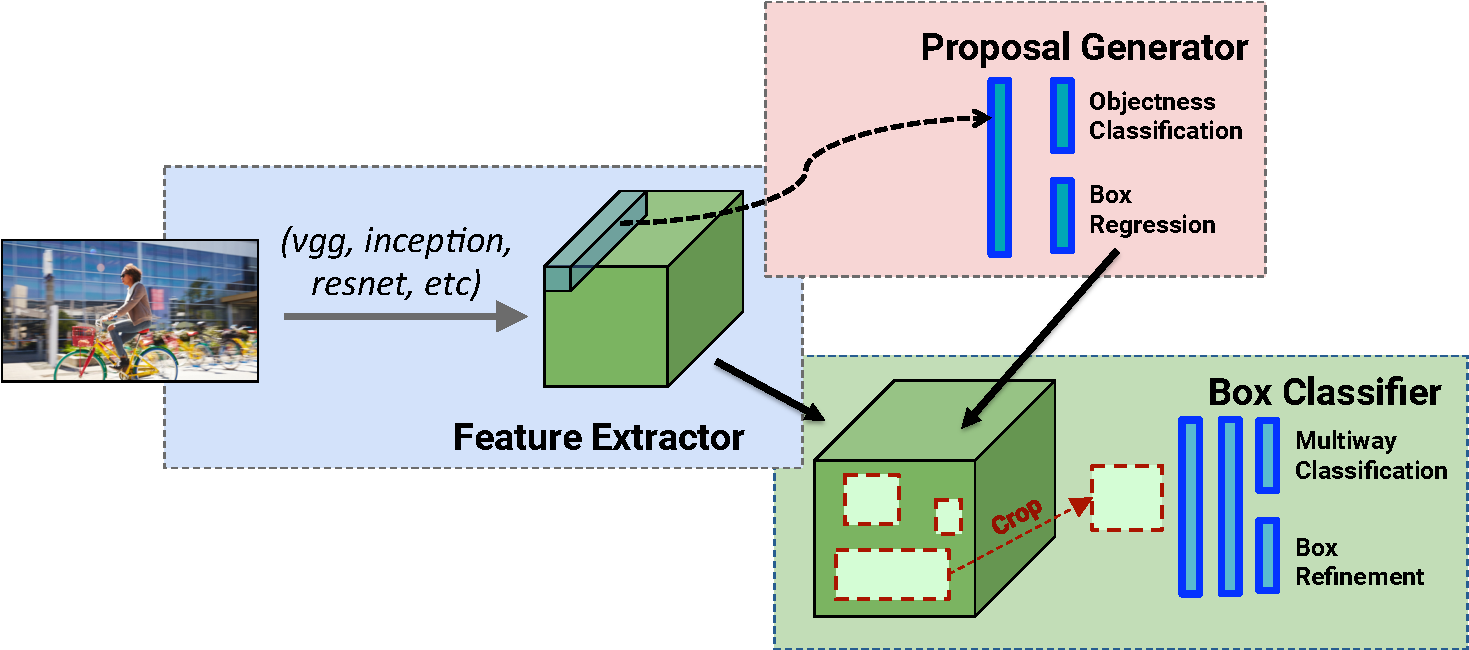
\includegraphics[width=0.85\linewidth]{fasterrcnn_diagram.pdf}
		\caption[The \FRCNN{} architecture]{The \FRCNN{} architecture \citep[credit to][]{detection_benchmark}
		\label{fig:faster_rcnn}
		}
	\end{figure}

	The task of object detection builds upon that of image classification since architectures based on region proposals (see \autoref{sec:related_detection}) can be seen as a two stage algorithm: the first part extracts possible object bounding boxes as a sub-image of the input, while the second one predicts the class associated with each candidate. It is of no surprise then that object detection greatly benefits from the super-human accuracy of deep neural networks \citep{superhuman_classif}. We chose to pair the \FRCNN{} detection architecture with the \RESNET{} feature extractor \citep{resnet}, since this has been proved to give a good trade-off between speed and detection accuracy on the standard challenge of ILSCVR \citep{detection_benchmark}. In what follows we present the main building blocks of this architecture.

	%----------------------------------------------------------------------------------------

	\subsection{Feature extraction}\label{sec:resnet}
		In order to perform detection on an input image, we first need to extract representative high-level features from the raw pixel values. To this end, we employ the \RESNET{} convolutional architecture which has won many competitions in classification, detection and segmentation.

		The novelty of this approach relies in forcing the network to learn a \emph{residual} mapping \(\mathcal{F}(\ve{x}) := \mathcal{H}(\ve{x}) - \ve{x}\), where \(\mathcal{H}(\ve{x})\) represents a desired mapping from input \(\ve{x}\), which is to be fit through a few stacked layers (\autoref{fig:resnet} left). This comes from the observation that the optimal function to be learnt could be closer to the identity mapping than to a zero mapping. Therefore, the new formulation eases the job of the optimiser since it only has to find perturbations around the identity mapping, rather than learn a completely new function.
		% http://www.robots.ox.ac.uk/~vgg/publications/2015/Jaderberg15b/jaderberg15b.pdf gives a good started about many things, including how ConvNets work

		Moreover, in order to keep the number of parameters as small as possible and have reasonable training times for very deep architectures (101 layers), standard convolutions are replaced by bottleneck-blocks of convolutions (\autoref{fig:resnet} right). Such blocks are formed by concatenating a \(1 \times 1\) convolutional layer at each end of the \(3 \times 3\) layer. The ``prefix'' layer reduces the number of filters while the ``suffix'' one increases it back, thus reducing the computational cost of the heavier middle layer.

		\begin{figure}
			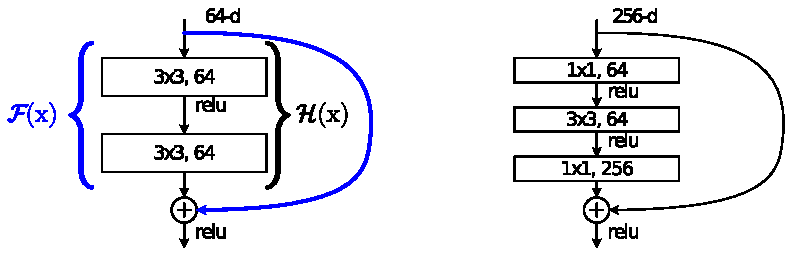
\includegraphics[width=0.85\linewidth]{resnet_blue}
			\caption[ResNet blocks]{
				The left part represents a normal ResNet block which forces the network to learn the residual mapping \(\mathcal{F}(\ve{x}) := \mathcal{H}(\ve{x}) - \ve{x}\) through the skip connection shown in blue. The right part shows a ``bottleneck'' block used in \RESNET{}.

				\raggedleft{\citep[credit to][]{resnet}}
				\label{fig:resnet}
			}
		\end{figure}

	%----------------------------------------------------------------------------------------

	\subsection{Region proposal network}\label{sec:frcnn_rpn}
		In order to bring the inference speed closer to real-time, \FRCNN{} improves on the bottleneck of previous approaches, namely the proposal of object candidates. Instead of relying on highly-engineered low-level features of super-pixels, the architecture reuses the convolutional feature map generated for the region classification step.

		This is achieved through another small, fully-convolutional network which is slid along the final layer of the feature map. The window at each location is projected into a lower dimensional feature that is used to predict \(k\) region bounds as well as \(k\) ``objectness'' scores. Each predicted region \(k_i\) is encoded as 4 coordinates \(\ve{t}_i = (x, y, w, h)_i\) that define the bounding box \emph{relative} to a set of predefined boxes called \emph{anchors}. This mechanism allows the detection of multiple scales and aspect ratios in one pass through the network, thus avoiding the need of image pyramids and further reducing the computational cost.

		For training the RPN, the following loss function has to be minimised:
		\begin{equation*}\label{eq:rpn_loss}
		L(\ve{p}_i, \ve{t}_i) =
			\frac{1}{N_{\cls}}\sum_i L_{\cls}(\ve{p}_i, \ve{p}^{*}_i)
			+ \lambda\frac{1}{N_{\reg}}\sum_i  \ve{p}^{*}_i L_{\reg}(\ve{t}_i, \ve{t}^{*}_i);
		\end{equation*}
		\(\ve{p}_i\) represents the probability that anchor \(i\) is an object; \(\ve{p}^{*}_i\) is the label of this anchor (\(1\) when it significantly overlaps a ground truth box) and \(\ve{t}_i, \ve{t}^{*}_i\) encode the anchor's and ground truth's coordinates, respectively.

		The loss jointly minimised  the ``objectness'' classification term \(L_{\cls}\) for an anchor \(i\) in the minibatch and the bounding box regression term \(L_{\reg}\); the two are balanced by the hyper-parameter \(\lambda\). The regression term is only taken into account for positive anchors (\(p^{*}_i = 1\)), which are those overlapping a ground truth box with an Intersection-over-Union (\(\iou\)) ratio above threshold \(\tau_+ = 0.7\).

	%----------------------------------------------------------------------------------------

	\subsection{Training}\label{sec:frcnn_train}
		In addition to generating object candidates with the RPN, the \FRCNN{} architecture also needs to classify the generated proposals. For this, it uses the Fast R-CNN architecture and trains both of them at the same time, as shown in \autoref{fig:faster_rcnn}. The forward pass generates box proposals that the classifier considers to be fixed for its training. This easy implementation ignores the gradients with regards to the coordinates of the proposal boxes, so it is only an approximation of the joint training procedure. However, its results are close to those obtained by alternating the training of the two networks, while being significantly faster.

		Instead of training the whole architecture from scratch, we gain significant time by using transfer learning and starting with a model that performs well on the ImageNet challenge. We replace its final softmax layer so that it only predicts among our two classes of interest: \texttt{text} or \texttt{background}.

		We hypothesize that the object / not-object distinction is easier to make for text on white background documents than it is for an ImageNet object in the wild. Therefore, we set hyperparameter \(\lambda = 2\) in order to give preference to the box regression loss. Moreover, in order to account for text's wide aspect ratio and relatively constant height in our documents, we change the default anchors to be similarly wide (ratios \(\{2, 4, 6, 8, 10\}\)) and with a limited set of scales (heights of \(\{50, 75, 100\}\)px). This further helps the box regression part to converge.

		We use the stochastic gradient descent (SGD) optimiser with momentum which updates the weights \(\ve{W}\) of the network using an exponential moving average of the gradients:\[
		\begin{split}
			\ve{V}_t &= \beta \ve{V}_{t-1} + (1-\beta) \nabla_w L (\ve{W}, \ve{X}, \ve{y}),\\
			\ve{W} &= \ve{W} - \alpha \ve{V}_t,
		\end{split}
		\]
		where \(\alpha\) is the learning rate and \(\beta\) is the momentum value. We use \(\beta = 0.9\) and a step decay schedule for the learning rate \[
			\alpha = \alpha_0 * 0.3 ^ {\floor{\frac{\mathit{step}}{1000}}},
		\]
		which starts with the initial learning rate \(\alpha_0 = 0.003\) and decreases it every 1000 steps.

		We feed the network one image at a time, resized such that its shorter side is 600px wide. Note, however, that a minibatch is formed of bounding boxes, so many candidates can be generated from a single input image and a set of anchors. Several hyper-parameters control the composition of the batches:
		\begin{description}
			\item[number of proposals (\(\mathit{value} = 300\))] How many object proposals are generated in each batch.

			\item[positive to negative ratio (\(\mathit{value} = 0.5\))] For a robust classification and convergence of ``objectness'' score, it is important that examples of both positive and negative candidates are generated.

			\item[positive IoU threshold (\(\tau_{+} = 0.7\))] An anchor is considered positive when \(\mathit{overlap}(\mathit{anchor}, \mathit{truthBox}) > \tau_+\). While \(0.7\) could be considered low for text objects (see \autoref{fig:text_overlap_example}), setting this value too high in the early stages leads to a lower number of positive candidate and slows down convergence of \(L_{cls}\).

			\item[negative IoU threshold (\(\tau_{-} = 0.3\))] Similar to \(\tau_{+}\), but for marking candidates as negative examples.

			\item[NMS confidence threshold (\(\mathit{value} = 0.0\))] When a candidate has a low confidence score, we can suppress it from contributing to the loss. We effectively disable this filter because we want to force the network to give high-confidence predictions, therefore it should learn from all examples.

			\item[NMS IoU threshold (\(\tau_{\textsc{nms}} = 0.7\))] When several proposals overlap each other, we should keep only one of them in the batch in order to increase proposal's diversity. This parameter controls when we can consider that a proposal is redundant to another one, in terms of their overlap.

		\end{description}

		On every experiment we monitor the training progress by intermittently evaluating the model on a validation dataset of images from the same category. The training is stopped once there is no significant improvement for more than two epochs, despite a decreasing learning rate.


%========================================================================================

\section{Connectionist Text Proposal Network}\label{sec:ctpn}
	% http://i.cs.hku.hk/~kykwong/publications/wliu_bmvc16.pdf This has a good simple explanation of ResNet and LSTM and what-not

	Once we established the feasibility of object detection techniques for our task via \FRCNN{}, we searched for improvements that could increase the quality of the detections. The rest of the section presents an extension to the previous architecture based on the work of \citet{CRNN} which is designed specifically for text detection.

	%----------------------------------------------------------------------------------------

	\subsection{RPN becomes CTPN}
		The main novelty of \FRCNN{} consisted of generating object candidates with a fast additional network based on a set of anchors which are combined in different scales and aspect ratios. This work builds on the observation that text does not have a closed boundary since it is composed of a sequence of letters and strokes. As such, a text ``object'' can have arbitrary width, which is difficult to accommodate with the standard anchor mechanism. The algorithm would need anchors of many different aspect ratios and even so, it would still be difficult to completely detect a line that is much longer than any of the ones in the training set.

		The \CTPN{} architecture proposes an ingenious solution: break down text objects into a series of adjacent boxes of constant-width and similar height; consequently, learn to predict a series of anchors that respect the same constraints, called \emph{fine-scale} proposals (\autoref{fig:ctpn_splitting}). Therefore, now the box regression is only concerned with the anchor's height \(h\), since the width is fixed and the RPN only has to learn text-specific features of a reduced bounding box of size \(h \times 16\).

		While the above is a clever twist on the original RPN, the merging of fine-scale proposals requires high-confidence outputs for all candidates in a series, i.e. for all boxes on the same line; otherwise it easily results in a segmented prediction. This is problematic especially when we want to detect multiple words as a single sequence on a line (\autoref{fig:ctpn_merging}), since each box is judged independently, based on its contents. As a solution, the series aspect should be exploited, and box prediction should make use of the context. To this end, the text proposal network is enhanced with a bi-directional LSTM layer
			\footnote{We will detail the inner workings of a similar LSTM layer in \autoref{sec:LSTM}}
		that sits of top of the sliding window network and propagates context between multiple predictions (\autoref{fig:ctpn_arch}). In this way, the network provides more consistency both for the confidence and for the heights of the boxes.

		A final refinement mentioned in the original paper consists of a regression of side margins of the first and last anchors on a detected line. Since we achieved good results without this part, we postponed its implementation for future improvements. As such, the loss function becomes almost identical to the RPN loss:
		\begin{equation*}\label{eq:ctpn_loss}
		L(\ve{p}_i, \ve{v}_i) =
			\frac{1}{N_{\cls}}\sum_i L_{\cls}(\ve{p}_i, \ve{p}^{*}_i)
			+ \lambda\frac{1}{N_{\reg}}\sum_j L_{\reg}(\ve{v}_j, \ve{v}^{*}_j),
		\end{equation*}
		except for the regression loss \(L_{\reg}\) which now only regresses a pair of coordinates, the centre and the height \(\ve{v}_j = \{v_c, v_h\}\) of the \(j\)-th anchor from the predefined set.


		\begin{figure}
			\begin{subfigure}[c]{.69\linewidth}
				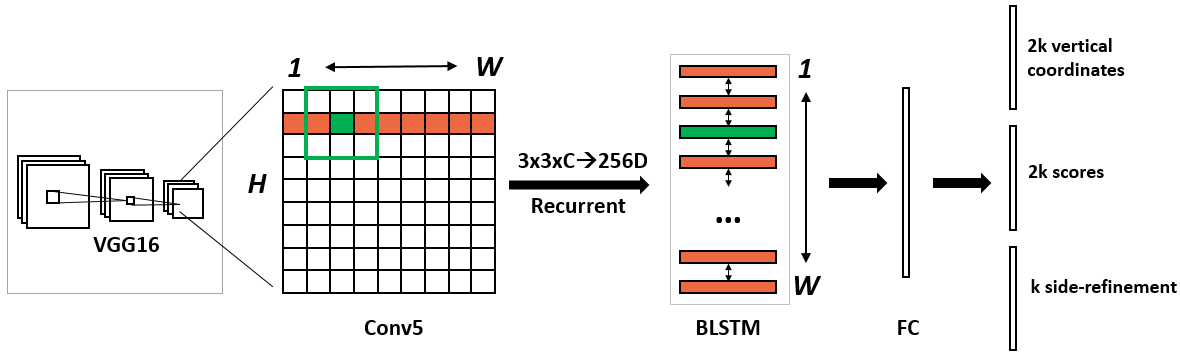
\includegraphics{ctpn_architecture}
				\caption{Overview \citep{ctpn}}\label{fig:ctpn_arch}
			\end{subfigure}
			\begin{subfigure}[c]{.30\linewidth}
				\begin{subfigure}{\linewidth}
					
\includegraphics{ctpn_orig}
					
\includegraphics{ctpn_split}
					\caption{Box splitting}\label{fig:ctpn_splitting}
				\end{subfigure}
				\par\bigskip
				\begin{subfigure}{\linewidth}
					
\includegraphics{ctpn_recon_fine}
					
\includegraphics{ctpn_recon_merged}
					\caption{Box merging}\label{fig:ctpn_merging}
				\end{subfigure}
			\end{subfigure}
			\caption[The \CTPN{} architecture]{The Connectionist Text Proposal Network:

			\subref{fig:ctpn_arch} The architecture comprises of the VGG feature extractor, succeeded by a fully-convolutional network coupled with an LSTM for fine-scale proposals.

 			\subref{fig:ctpn_splitting} Original bounding box and the corresponding series of equal width boxes.

 			\subref{fig:ctpn_merging} Predicted fine-scale proposals and the resulting bounding boxes. Note the limited merging due to missing proposals.
			}
		\end{figure}

	%----------------------------------------------------------------------------------------

	\subsection{Training}
		The original paper does not mention how fine-scale proposals are generated from the original bounding boxes, nor how they are merged to predict a large box. We found this to be an important implementation detail as it introduces a hyper-parameter \(\tau_{gap}\) which is a threshold for the maximum gap allowed between two neighbouring proposals. For example, in \autoref{fig:ctpn_merging} a small \(\tau_{gap}\) resulted in an overly-segmented of a word, whereas a too large \(\tau_{gap}\) would have merged the words together. Whether this is desired or not depends on the context. We have set \(\tau_{gap} = 24\)px, which is \(1.5\) times larger than the anchor width.

		Once the \CTPN{} predicts fine-scale proposals, these are classified into \texttt{text} or \texttt{back\-ground} by the same Fast R-CNN core as before. However, in this case we use a different feature extractor, namely the VGG network \citep{VGG}, in order to reproduce the setup of the original work. As in the previous case, we do not train from scratch but instead we start with the weights provided by the authors, who used 3000 images of text in the wild.

		We observed that a large number of the generated anchors were meaningless in our context due to little variation of text height. Therefore, we changed the default set of anchors to use only 3 different heights: \(\{10, 16, 23\}\) pixels which correspond to the most common ground truth heights after resizing the image to be 600px wide. This reduced the iteration time more than three times and also resulted in faster convergence of the training.

		We minimised the loss function using the Adam optimiser \citep{adam}, with an initial learning rate \(\lambda = 0.0001\). Furthermore, we used \(L_2\) regulariser with balancing weight \(\lambda_{L2} = 0.0005\).

%========================================================================================


\section{Datasets and experiments}\label{sec:detection_experiments}
	%-- INTRO -------------------------------------------------------------------------------
		Given the large number of parameters in deep neural networks (\(\approx 6 \times 10^8\) for \RESNET{}), it is clear that large amounts of training data are needed to train our architectures. Since this is lacking for our project, we must find alternative sources of handwritten text, ideally in the same language as the documents, i.e. French. Moreover, as was noted in \autoref{sec:challenges}, our documents have a difficult, albeit well-defined format, and less than optimal quality.

		The RIMES database \citep{rimes} is the result of a huge data collection effort by the French ministries of defense and research, which was set up in order to create a new, consistent database of handwritten text. Its novelty was that it also included mixed pages, with handwritten and printed text, as well as being almost completely unconstrained with regards to the content of the text.	It contains more than \(50\,000\) handwritten words that are made available individually, or in lines (more than \(9000\)), or in paragraphs (more than \(1500\)). We will base most of our experiments on this collection of handwritten text, though the following sections will detail different ways of adapting it to our use case. Additionally, we will also use our handwriting generator from \autoref{sec:generator} to analyse the influence of the training set and to overcome limitations of the RIMES database.

	%----------------------------------------------------------------------------------------

	\subsection{Evaluation framework}\label{sec:detection_eval}
		Before delving deeper into the details of our experiments, it is necessary to introduce requirements of the task and measures for quantifying their achievement. This section introduces one such measure that we will use for quickly assessing the outcome of an experiment. An in-depth evaluation will be carried on in \autoref{sec:detection_results}.

		Judging a detection result via a single number is a very difficult task, since the lack of a \emph{cost} associated with a false positive requires a trade-off between different types of errors. Standard object detection challenges such as PASCAL VOC \citep{pascal_voc} required participants to rank their results by a score, commonly referred to as \emph{confidence}. This allows the evaluation of a trade-off between false positives and false negatives by assessing the area under the precision/recall curve. To this end, the Average Precision is used:\[
			\operatorname{AP} = \frac{1}{11} \sum_{r \in [0,1]} p(r),
		\] which is the mean of precisions \(p\) computed at eleven equally spaced recall values \(r \in [0,1]\).

		Two essential observations need to be made. First, a great importance is given to the confidence score, since recall and precision are defined by only considering examples ranked above a given rank. Second, the measure does \emph{not} define what a positive result means. For object detection, a predicted bounding box \(B^p\) is positively mapped to \mbox{ground truth} box \(B^{gt}\) when their overlap exceeds a given threshold \(\tau\). The overlap is defined as \[
			\iou(B^p, B^{gt}) = \frac{\mathit{area}(B^p \cap B^{gt})}{\mathit{area}(B^p \cup B^{gt})}.
		\] In general, the threshold is set at \(\tau = 0.5\) and the measure is denoted by \(\AP\).

		Since text detection is a particular case of object detection, it generally subscribes to the same evaluation criteria. However, text is more than a simple object with binary presence; it consists of a sequence of characters, all of which are mandatory and of \emph{equal} importance to the meaning. This is in contrast to objects in general images such as those in the PASCAL VOC database. While such objects also admit a hierarchical structure (e.g.\ a cat has eyes, ears, legs, tail etc.), the presence of their sub-elements is not always mandatory; on the contrary, a subset of composing elements is almost always hidden due to self occlusions. This allows some partial detections to be considered valid in the context of objects (see \autoref{fig:cindy}). Text detection cannot afford such flexibility, since we aim to use the detections in a subsequent step of transcription. This requires that bounding boxes include all relevant text and, ideally, no other text fragments such as parts of the line above or below (see \autoref{fig:text_overlap_example}).

		Considering that in our documents text lines are close to each other, we demand the detections to be as tight as possible around the text. However, given the lack of a baseline in such challenging documents, we will base our intermediate decisions on the standard measure of \(\AP\). This allows us to compare our text detection models with their object detection counterparts.

		\subsubsection*{Test data}\label{sec:detection_test_data}

		Given that our approaches rely on transferring knowledge from generated data, we need an objective way of comparing their performance. To this end, we constructed a \ds{Test} dataset to provide ground truth labels on real-world data. This consists of 26 annotated statements which amount to approximately 1400 bounding boxes.

		\begin{figure}
			\begin{subfigure}[b]{0.49\linewidth}
				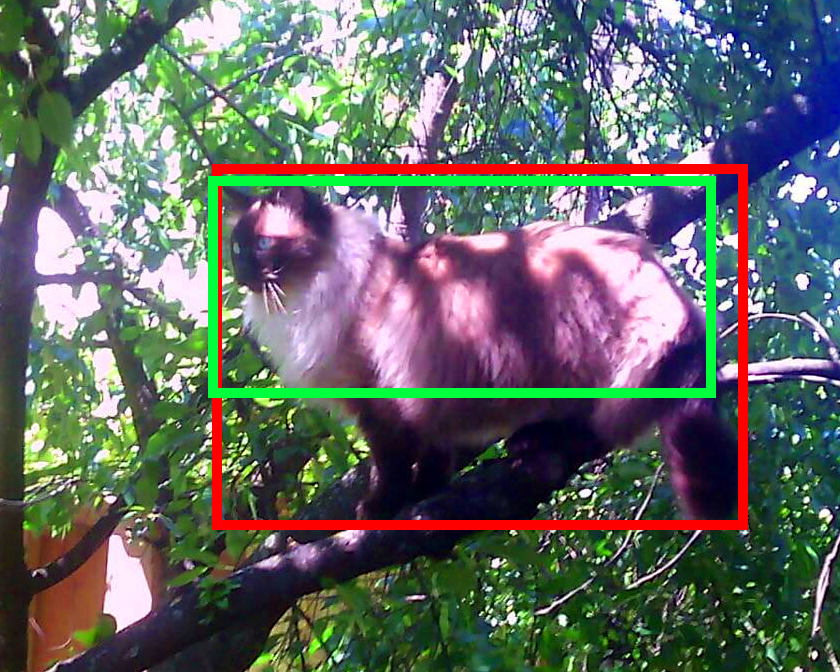
\includegraphics{cindy}
				\caption{\label{fig:cindy}}
			\end{subfigure}
			\begin{subfigure}[b]{0.49\linewidth}
				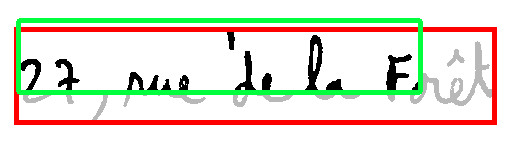
\includegraphics{text_iou}
				\vspace{2em} % no idea why this works. it was supposed to add space *between* the images, but oh well...
				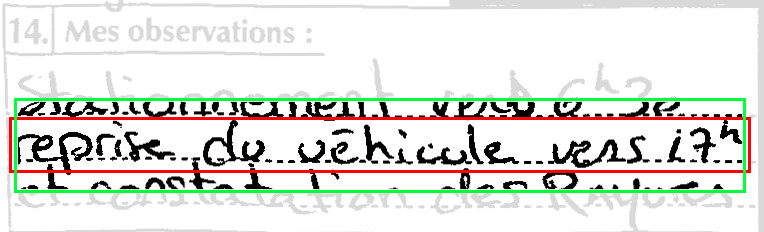
\includegraphics{text2_iou}
				\caption{\label{fig:text_overlap_example}}
			\end{subfigure}
			\caption[Overlap examples]{Overlap examples: red shows ground truth; green shows detection. In all cases \(\iou = 0.55\). While this is a valid detection threshold for a normal object, it is unsatisfactory for text recognition.
			}
			\label{fig:overlap_example}
		\end{figure}

	%----------------------------------------------------------------------------------------

	\subsection{Collage of paragraphs}
		\subsubsection*{\ds{Collage} dataset}

			For the first training session, we used images of paragraphs from the database along with their segmentation into lines as labels. To make them resemble the format of the documents, we juxtaposed two or three paragraphs picked at random from the database. These were corrected for rotation and augmented with borders to look similar to the sections of a document (\autoref{fig:collage}). We generated \(3500\) examples for training and \(500\) for validation.

		%........................................................................................

		\subsubsection*{Outcome}

			A \FRCNN{} model trained on this dataset converged rather quickly, in \(\approx 8000\) iterations. On its validation data, the model achieves a remarkably high performance, with \mbox{\(\AP = 0.96\)}. Note that the best performance of any model in object detection so far is \(\AP \simeq 0.73\), which clearly indicates that the task is very easy for the chosen model. However, the performance does not extend to the \ds{Test} dataset, achieving only \(\AP = 0.02\). This highlights the differences between the training and the test datasets. The most likely cause of the performance drop is the presence of additional elements in a real document, such as printed text and indicator lines, which do not exist in the training images. Therefore, the negative anchors generated by the algorithm are inevitably white boxes. In addition, the model regresses the anchor sizes to predict boxes of shape similar to the input lines. These display little variation in width and are, in general, much wider than the text fields of a document.

		\begin{figure}
			\begin{subfigure}[c]{\textwidth}
				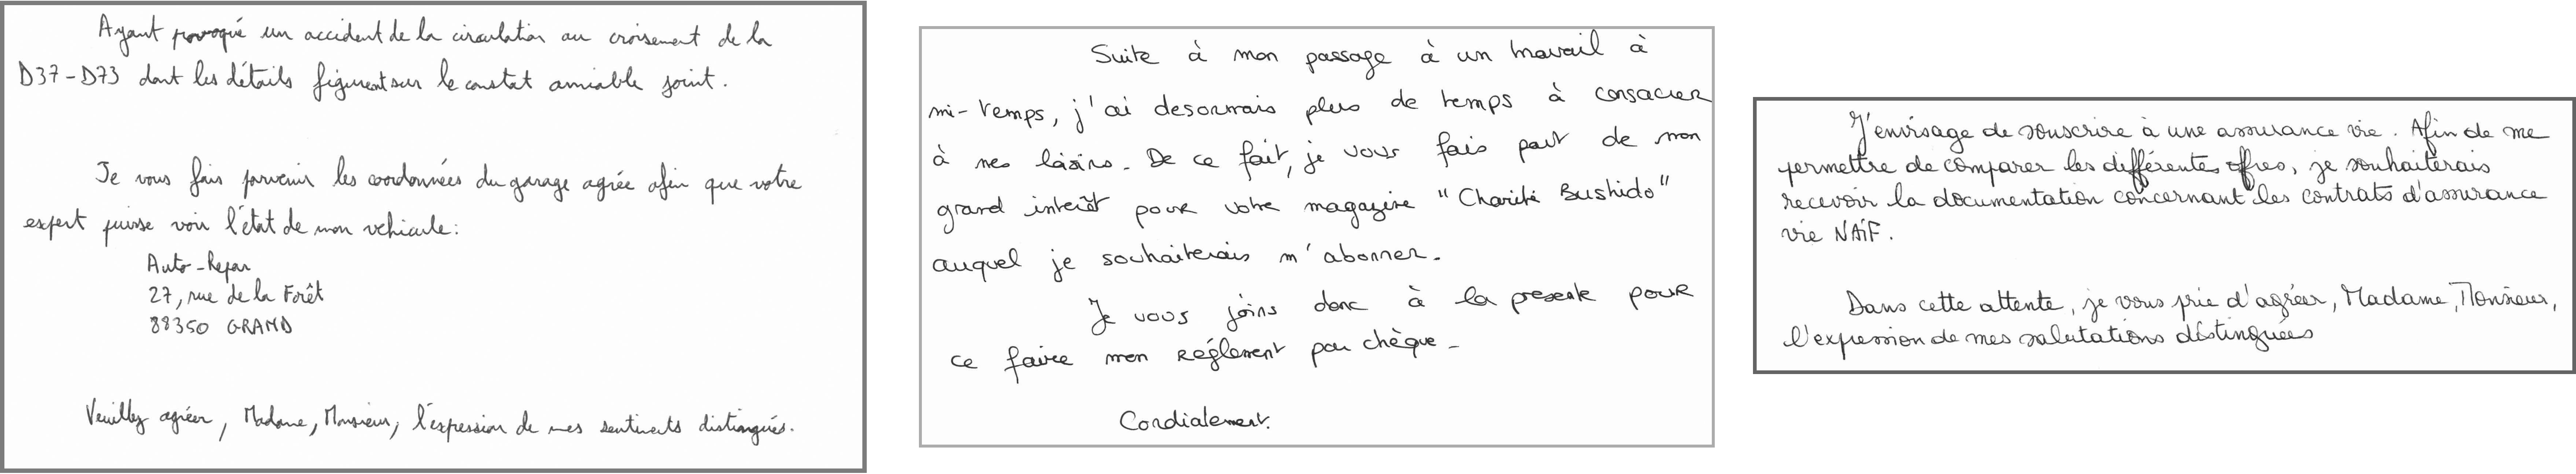
\includegraphics{collage_3}
				\caption{}
				\label{sfig:collage_clean}
			\end{subfigure}
			\vspace{1em}

			\begin{subfigure}[c]{\textwidth}
				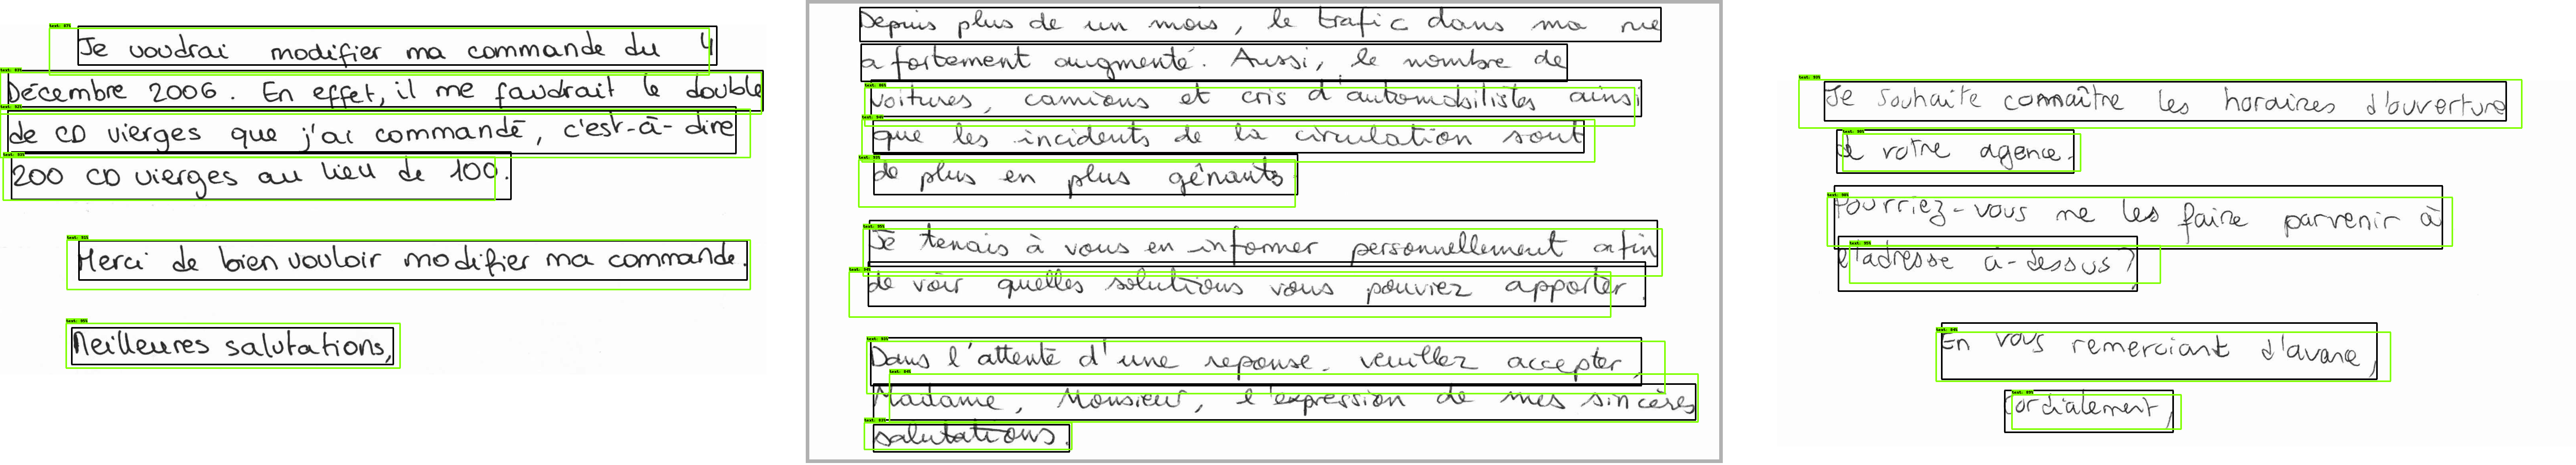
\includegraphics{collage_3_detected}
				\caption{}
				\label{sfig:collage_detect}
			\end{subfigure}
			\caption[\ds{Collage} dataset]{
				The \ds{Collage} dataset.
				\subref{sfig:collage_clean}: Example of generated collage document with 3 juxtaposed paragraphs.
				\subref{sfig:collage_detect}: The detection performed on such a document, with ground truth in black and detection result in green.
			}
			\label{fig:collage}
		\end{figure}

	%----------------------------------------------------------------------------------------

	\subsection{RIMES-filled templates}
		%........................................................................................
		% subsubsection: general description

			To address the limitations of the \ds{Collage} dataset and allow the model to learn more complex patterns, we propose to generate images which resemble more the real documents. To this end, we fill accident statement templates of 4 different styles with handwritten text from a database. This results in realistic looking documents while saving the high cost of manual labelling.

		%........................................................................................

		\subsubsection*{\ds{Template} and \ds{Template_bin} datasets}\label{sec:rimes_template}
			A template is formed by adding input placeholders to an empty document (\autoref{fig:template}). These correspond to the standard places that the users need to fill as well as non-standard places where users regularly add information. To increase the variation of the data, only a subset of the placeholders are filled on each template instance and the input text is shifted horizontally inside the placeholder by a random amount. We investigate two possible text sources for filling the templates.

			\begin{figure}
				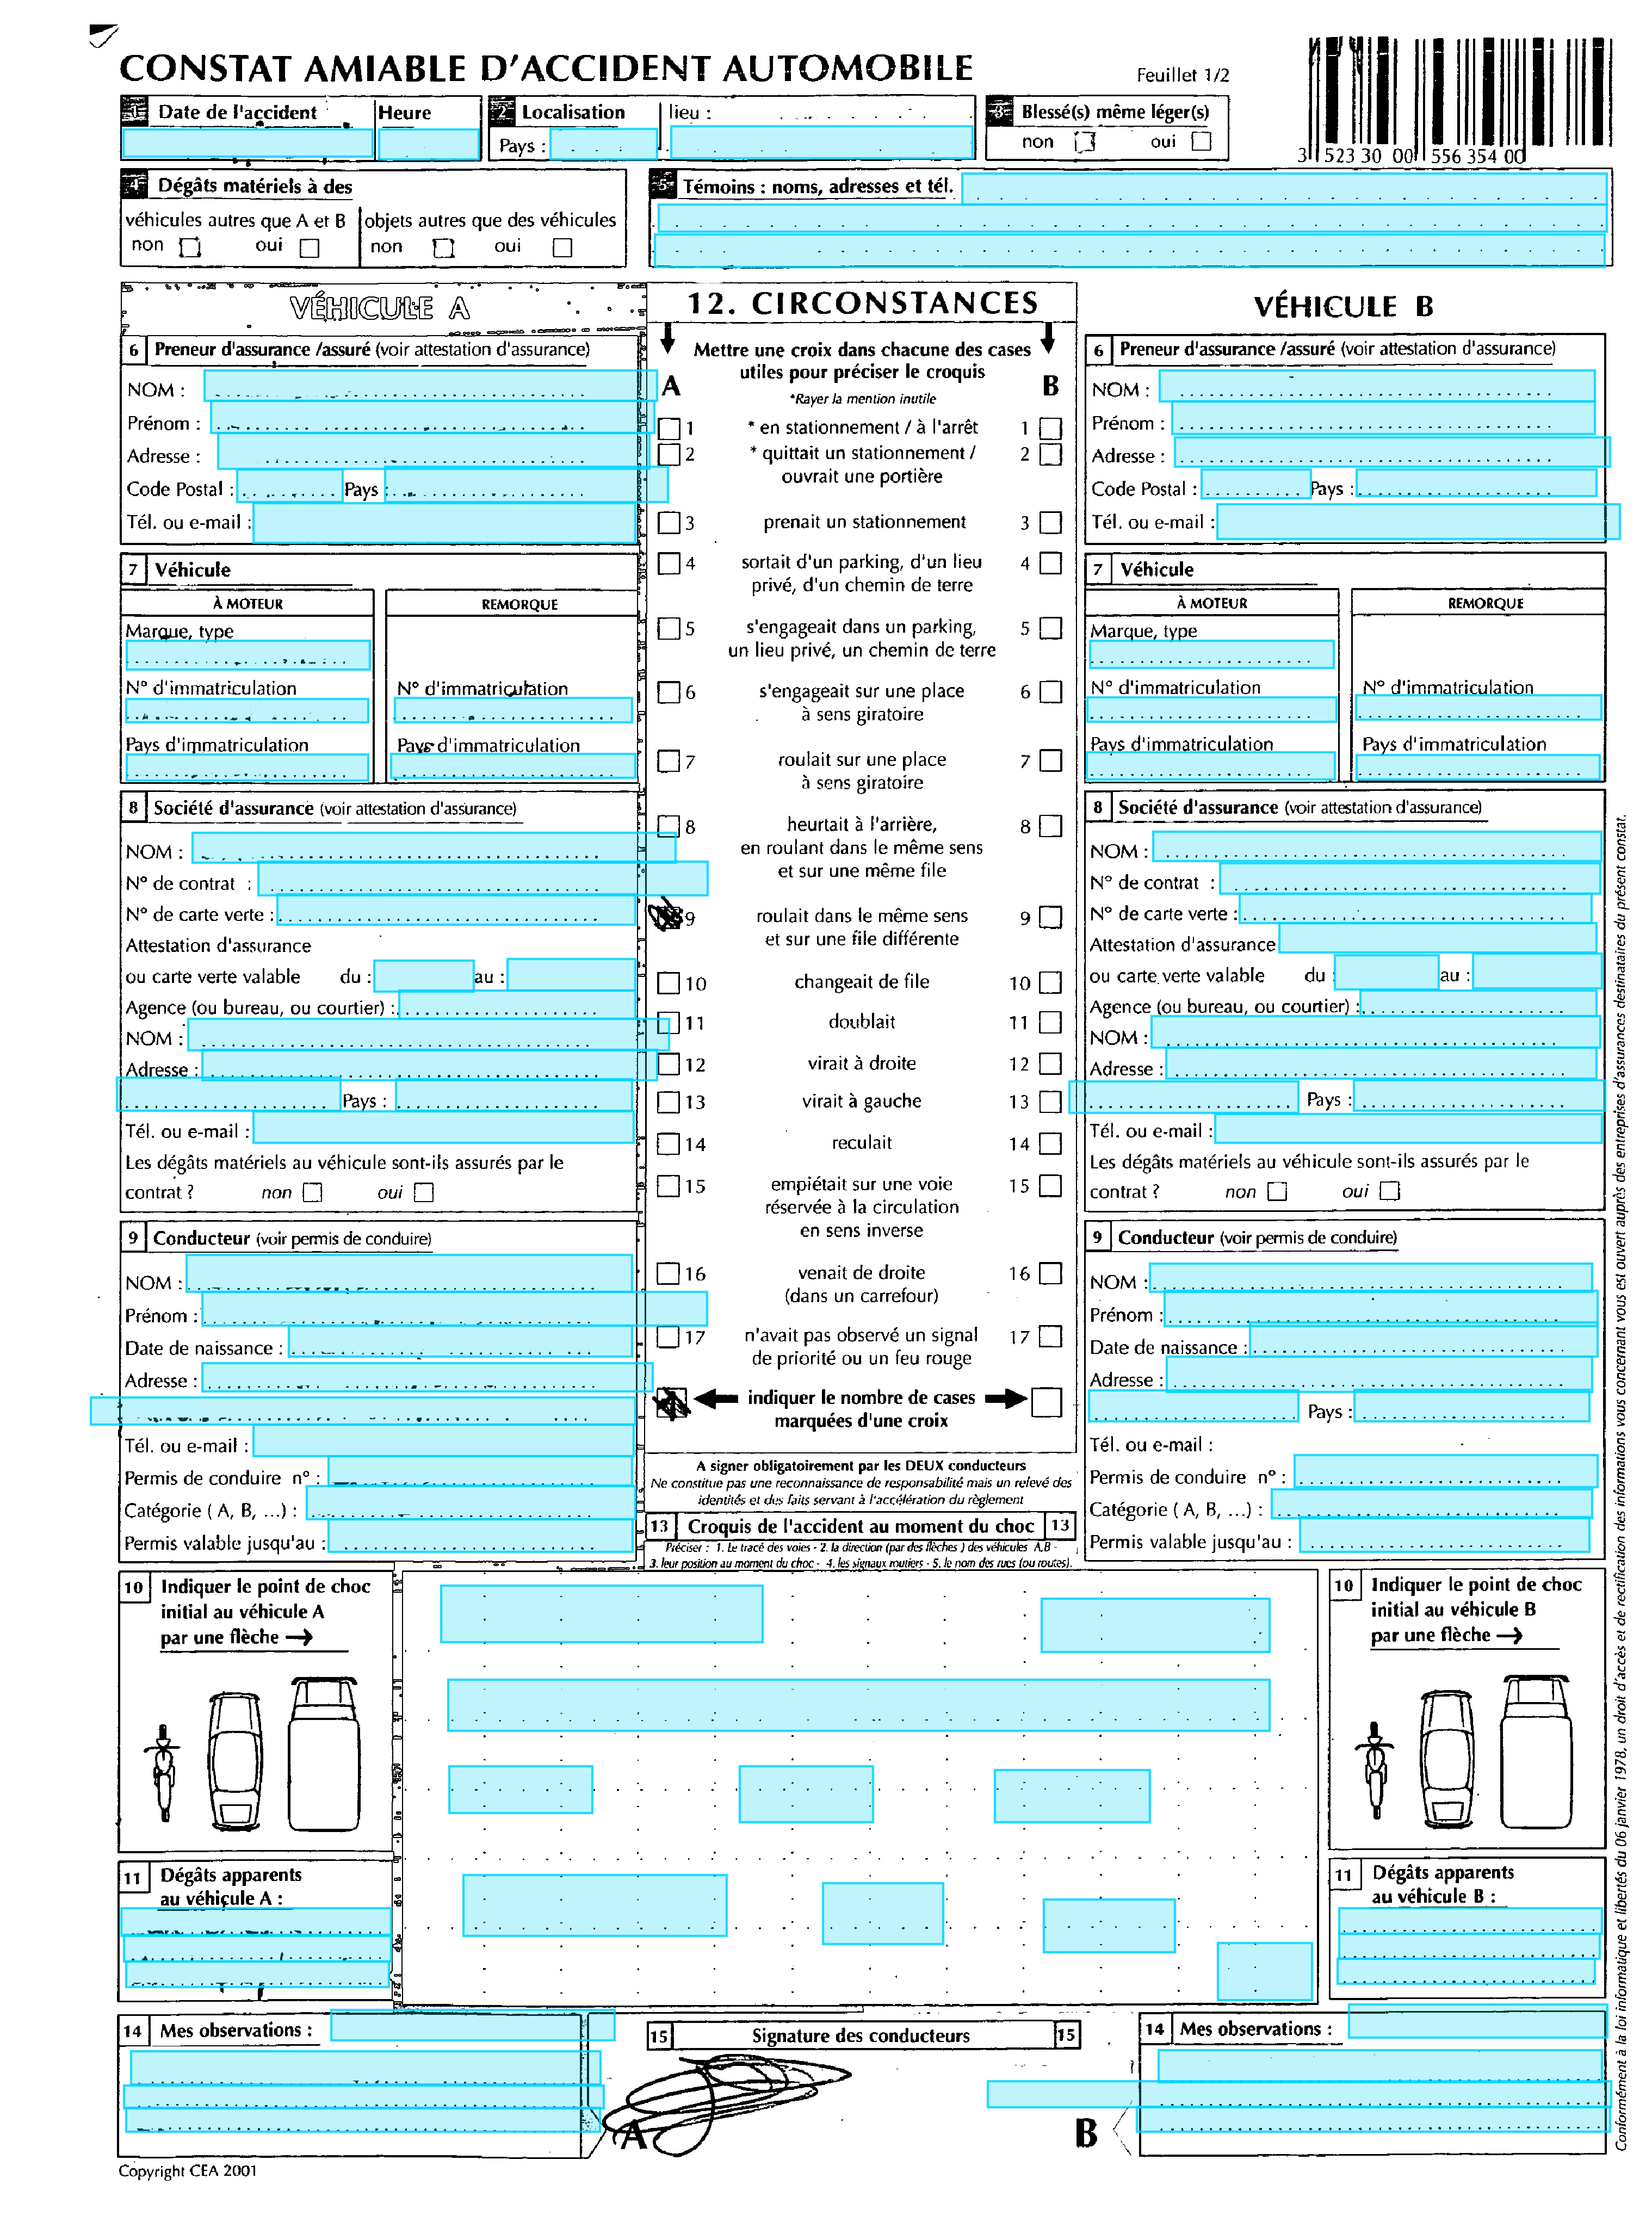
\includegraphics{template_empty}
				\caption[Document template]{An empty document template. Note that the placeholders are slightly bigger than the location for text entry in order to allow text that goes out of bounds. Also, there are placeholders in places that do not correspond to any field, which matches how people use these documents.}
				\label{fig:template}
			\end{figure}


			The first one consists of images of \emph{individual} words from the RIMES database. This has the advantage of tight bounding boxes around the text, which we established as an important criterion in \autoref{sec:detection_eval}. Also, it allows us to keep the ground truth text associated with each box, which will also make them useful for the transcription step. On the other hand, this source also poses some problems. First, words are generally shorter than the placeholders, so we would need to concatenate several words to resemble the real data. Since the word order was lost when constructing the database, this has the disadvantage that lines formed in this way do not follow any sentence structure. Furthermore, words with ascenders and descenders would need to be aligned to their baseline, which is especially difficult to estimate for short words. Finally, handwriting styles from multiple authors would be combined on the same line and in the same document section.

			The second source of text consists of images of text lines from the same database. This addresses the problems of word concatenation, but introduces another difficulty: the lines are usually longer than the placeholders, so they need to be cut. However, thinking forward about the text transcription part, we immediately realise that in order to have reliable \((\mathtt{image}, \mathtt{label})\) pairs, we must ensure line images are split \emph{only between the words}. We use the following algorithm to detect good splitting points in image \(\ve{I}\): % https://tex.stackexchange.com/questions/172399/how-to-write-sentences-in-an-algorithm-in-latex https://tex.stackexchange.com/questions/142922/how-to-align-text-within-an-algorithm-environment
			\noindent\begin{minipage}{\linewidth}
			\begin{enumerate}
				\item use the line transcription labels to find the number of words \(n\)
				\item project the image columns horizontally, accumulating their sum into \[
					\ve{p}_c = \sum_{r = 1..H }\ve{I}_{r,c}
				\]
				\item find the continuous runs of zero \(\ve{z} = \{ (i, j) \mid \ve{p}_k = 0, \forall k \in [i, j] \}\); these correspond to gaps between letters (marked in red in \autoref{fig:baseline_ok})
				\item take \(n\) widest gaps \(\ve{z}'\) from \(\ve{z}\), where the gap width \(w := j - i\)
				\item split at columns \(c_k = \frac{j_k - i_k}{2}, \forall (i_k, j_k) \in \ve{z}'\).
			\end{enumerate}
			\end{minipage}
			\\

			To avoid placeholders filled with very short words, we add multiple words to the same placeholder until it is at least 70\% filled. Note that unlike the first text source, these words come in order from the original line, split by the above algorithm. Moreover, lines come sequentially from the same paragraph, so there is writer consistency for a good part of a template, just like in the real world.

		%........................................................................................

		\subsubsection*{Baseline detection}
			When humans fill a statement template, the baseline of their handwriting lies roughly on an indicated line.  We purposely set the placeholder's bottom edge on this line in the interest of aligning the text image in a similar manner. Then we use the following simple procedure to find the baseline row \(r_b\) of a text image \(\ve{I}\) of size \(H \times W\) (\autoref{fig:baseline}):
			\noindent\begin{minipage}{\linewidth}
			\begin{enumerate}
				\item project the rows of the image by averaging the pixel values: \[
					\ve{p}_r = \frac{1}{W} \sum_c I_{r,c}
				\]
				\item let \(m = \operatorname{median}(\ve{p})\)
				\item the baseline is the first row \(r_b\) where \(\ve{p}_{r_b} > m\), \(b = H..1\).
			\end{enumerate}
			\end{minipage}\\

			The method above works well as long as a few assumptions hold. First, the text image has to be horizontal. In case it is not (see \autoref{fig:baseline_skewed}), we de-skew it by rotating with the average angle of Hough lines. Second, the input line has to be correctly segmented vertically. As a counter example, \autoref{fig:baseline_segmentation} shows that due to another text line present in the same image it is difficult to segment the words correctly. Fortunately, the database does not contain many examples that break these assumptions and we can reject tokens resulted from a failed segmentation based on their length.

			\begin{figure}
				\begin{subfigure}{\linewidth}
					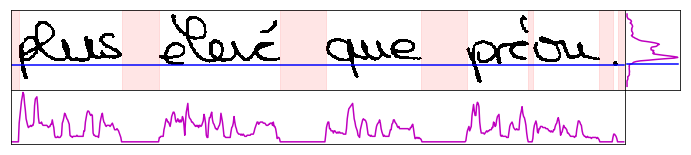
\includegraphics{baseline_ok}
					\caption{Good and clean horizontal image}
					\label{fig:baseline_ok}
				\end{subfigure}
				\bigskip

				\begin{subfigure}{\linewidth}
					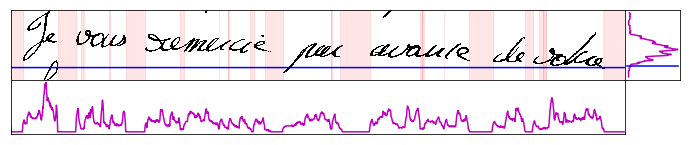
\includegraphics{baseline_skewed}
					\caption{Skewed image}
					\label{fig:baseline_skewed}
				\end{subfigure}
				\bigskip

				\begin{subfigure}{\linewidth}
					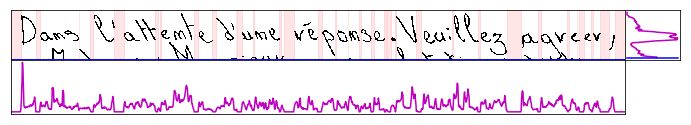
\includegraphics{baseline_segmentation}
					\caption{Badly segmented image, with slanted text}
					\label{fig:baseline_segmentation}
				\end{subfigure}
				\caption[Baseline and tokens]{Detection of the baseline and the tokens in a text image.}
				\label{fig:baseline}
			\end{figure}

		%........................................................................................

		\subsubsection*{Outcome}
			With the above techniques we generated 1000 templates for training, for a total of 50\,000 text examples; we will refer to this dataset as \ds{Template}. It became apparent that this task was appropriately more difficult than the \ds{Collage} dataset, as the validation performance was still improving after 35\,000 steps. However, due to a slow improvement rate, we stopped the training there, as we deemed the validation performance ``good enough'' for an experiment, at \(\AP \simeq 0.76\). Surprisingly though, the performance on the \ds{Test} dataset was essentially zero (\(\AP \simeq 0.007\)). A very close inspection of the generated data, in comparison to the test data, revealed a key difference between the two: the real-world documents are (almost) binarised, while the text from the RIMES database is not (\autoref{fig:template_gray_hist}). Convolutional neural networks should be robust to general appearance changes, especially when random contrast is used as a data augmentation technique. However, knowing that the first filters of CNNs correspond to edge extractors, we hypothesise that the disruption is given by the transitions from foreground (text) to background (white). In the case of RIMES, these are soft edges and only extreme contrast boosts can convert them into hard edges (\autoref{fig:template_gray_example}).

			\begin{figure}
				\begin{subfigure}{\linewidth}
					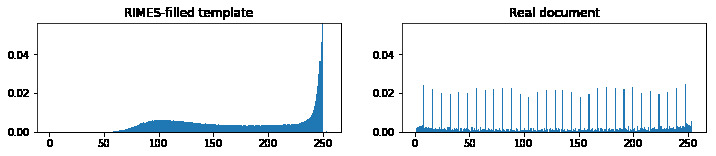
\includegraphics{template_hist}
					\caption[Template histograms]{
						Examples of normalised histograms with the extreme counts removed (0 and 255). The templates filled with text (left) present more shades of gray than a real document (right).  Moreover, only half of real documents present such a structure, the other half being completely binarised, i.e. with a completely empty histogram (after removing the background/foreground extremes).
					}
					\label{fig:template_gray_hist}
				\end{subfigure}
				\begin{subfigure}{\linewidth}
					
\includegraphics[width=.49\linewidth]{binarisation_template}
					
\includegraphics[width=.49\linewidth]{binarisation_real}
					\caption{In addition to being gray, text from the RIMES database has soft edges, while text from real documents has a hard transition from foreground to background.}
					\label{fig:template_gray_example}
				\end{subfigure}
				\caption{Differences between \ds{Template} and \ds{Test}}
				\label{fig:template_gray}
			\end{figure}

			We generated another dataset, \ds{Template_bin}, of same size as \ds{Template}, where we binarised text before pasting it into the documents (\autoref{fig:template_bin_detection}). Given the uniform illumination, a global thresholding technique worked well, with the threshold chosen by Otsu's method. The model trained on this dataset converged after 4500 steps and has a validation \(\AP \simeq 0.83 \). It also generalizes better than previous ones on the \ds{Test} dataset, with an \(\AP \simeq 0.37\).

			\begin{figure}
				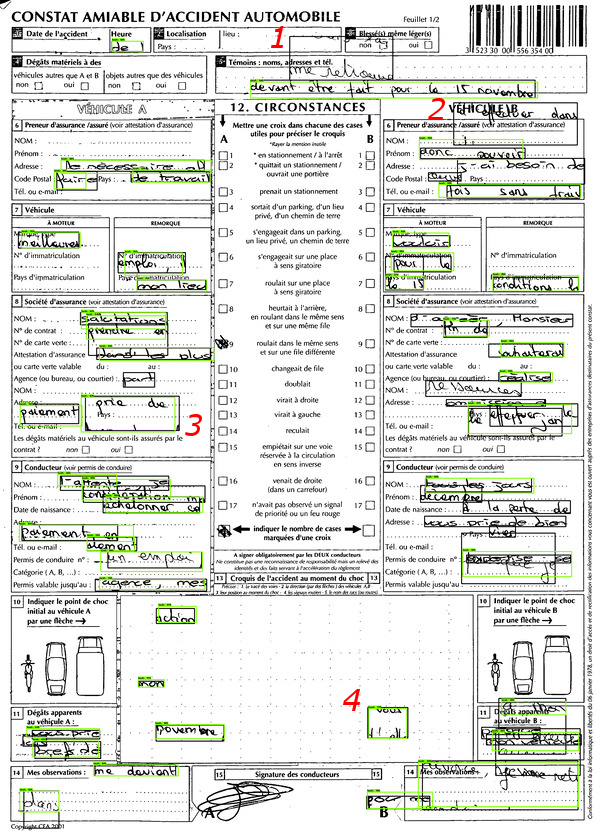
\includegraphics[height=.85\textheight]{template_bin_detection}
				\caption[\ds{Template_bin} example]{Example of template filled with binarised text from the RIMES database. Black shows ground truth boxes, and green the detection result. This particular example also presents some bad ground truth examples, marked by red numbers. Some of them are not detected (1, 2) while some are detected with high precision (3, 4). }
				\label{fig:template_bin_detection}
			\end{figure}

	%----------------------------------------------------------------------------------------
	\subsection{Generator-filled templates}
		As will be apparent from the results of the \FRCNN{} architecture (\autoref{sec:frcnn_results}), the model learnt to predict rather tall bounding boxes which are not representative for real documents. One reason for this is that we used the original height of text lines in order to avoid artefacts of interpolation in resizing. Additionally, the model picked up peculiarities of the training set, such as incorrectly segmented lines.

		%........................................................................................

		\subsubsection*{\ds{Template_gen} dataset}

			To overcome the above limitations, we used our text generator from \autoref{sec:generator} to fill templates as before. It produces coherent and realistic-looking text of given dimensions. This ensures the bounding boxes are always tight and a correct baseline is used for alignment inside the placeholder. Moreover, the height of the text is within the boundaries of the placeholder while keeping the binary distribution of pixels (i.e. avoiding interpolation). The sole possible disadvantage of this method is that we did not enforce a consistent style for all text pieces in a given section. Nevertheless, we realised this should bear a minimal influence on the detection since the algorithm is translation invariant and it scans the image left to right, top to bottom, not following the section order.

		%........................................................................................
		\subsubsection*{Outcome}

			This model was the fastest to converge of all, attaining a validation \(\AP = 0.98\) in approximately 3500 iterations. However, when visually inspecting a small detection sample of validation images at \(\mathit{step} = 3500\), we note a relatively low recall compared to expectations from previous model (\autoref{fig:gen_detection}). This could be explained by the complete separation of validation and training data, the two being generated with completely different text and sets of fonts. Additionally, we also note a higher than usual loss of the classification core, which means that the RPN learnt quickly to propose text-like boxes, but the classification network was not yet sure which ones correspond to handwriting. This is expected to a certain degree since printed and handwritten text are very similar in our documents. Finally, the apparent high performance despite the visually low recall highlights why a more in-depth analysis is needed.

			We further trained the model for another 4000 steps, until the classification loss also converged; the validation precision remained the same. At this point, we tested the model on the \ds{Test} set and noted approximately 10\% improvement over the previous best, with \(\AP = 0.47\).

			\begin{figure}
				% floatrow magic for having sidecaption https://tex.stackexchange.com/a/29144/76755
				\floatbox[{\capbeside\thisfloatsetup{capbesideposition={left,top},capbesidewidth=.48\linewidth}}]{figure}
				{
					\caption[\ds{Template_gen} detection]{Despite reporting almost perfect precision after 3500 steps, a \FRCNN{} model trained on \ds{Template_gen} dataset exhibits quite a low recall that is hard to explain. This small example shows similarly looking text; some of it was detected with maximal confidence, some of it was ignored. Black boxes represent ground truth and are \emph{not} part of the image. }
					\label{fig:gen_detection}
				}
				{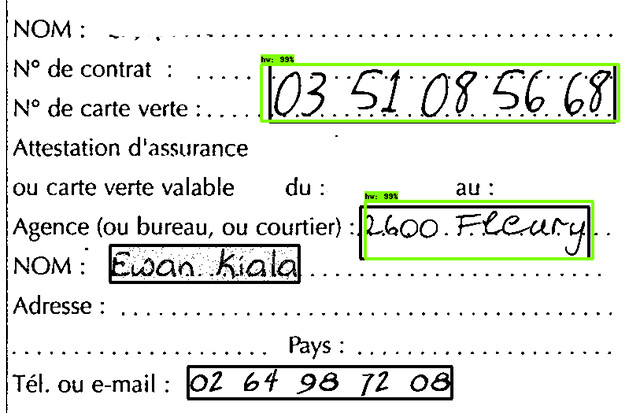
\includegraphics{gen_detection_no}}
			\end{figure}

	%----------------------------------------------------------------------------------------
	\subsection{CTPN test}
		Having proved the feasibility of general object detection architectures for our task, we started seeking further improvements by employing the text-specialised architecture of \CTPN{}. We build upon the previous progress and train directly on the dataset with best results so far, \ds{Template_gen}. The model converged after 10\,000 steps and achieved a validation \(\AP = 0.69\). Despite giving the best results visually on \ds{Test} dataset, it appears to perform worse than the best \FRCNN{} model, with \(\AP = 0.31\).


%========================================================================================


\section{In-depth evaluation}\label{sec:detection_results}
	% this evaluates text detection in 2 simple numbers (P, R), in terms of pixels: http://vision.soic.indiana.edu/papers/textevaluation2000das.pdf

	We have seen in the previous section that different combinations of architectures and training datasets achieve vastly different performances on real data. Moreover, as briefly discussed in \autoref{sec:detection_eval}, it is difficult to quantify them through a single number. This was also confirmed empirically when observing that intermediate models with high \(\AP\) scores gave subpar detections. Therefore, in what follows we will perform a more in-depth analysis of models' performance in the interest of finding the factors that contribute to improvement and choosing the most robust model.

	\Citet{objdet_performance} give an overview of different metrics that can be useful for detailed evaluation of object detection algorithms. We are interested in evaluating both the detection \emph{quantity}, as well as its \emph{quality}. However, these two measures are related, since the detection quantity depends on our quality requirements. We could overcome this tight connection by performing evaluation at a higher level through a \emph{goal-directed} approach. In such a case, the text locating algorithms would be judged by the recognition rate they achieve when coupled with a text recogniser. However, this would introduce another dependency in the system and, to the best of our knowledge, no robust system exists yet for handwriting.

	We reiterate the main concerns for this evaluation:
	\begin{description}
		\item[high recall] A good model should find most of the ground truth boxes.
		\item[precise detection] Bounding boxes that correspond to ground truth should be tight around the text. Note this is different from the overall precision in general (see next point).
		\item[variable general precision] We are forgiving about false positive detections, i.e.\ bounding boxes that do not correspond to any ground truth, since we expect the recogniser to fail on these, thus acting as a filter.
	\end{description}

	\subsection{Faster R-CNN}\label{sec:frcnn_results}
		\urldef{\cocoURL}\url{http://cocodataset.org/#detections-challenge2017}

		We started our training with a model pre-trained for the COCO object detection challenge\footnote{Common Objects in Context \cocoURL}, which claimed an \(\AP \simeq 0.32\). We have reached a similar performance on our \ds{Test} dataset. On the one hand, further improvements should be possible since our task has less classes and less background variation. On the other hand, what we call \emph{background} actually consists of printed text, which is very similar in structure to the handwritten one, especially if both are upper case. We will consider this as a baseline and we will inspect how the training data affects the performance.

		%........................................................................................
		\subsubsection*{Metrics}
			In a first phase, we use the confidence scores to rank the detections and we inspect the variation of recall while varying the score threshold (\autoref{fig:frcnn_results} top). Recall at threshold \(\tau\) is defined as the ratio between the number of true positives and the number of \mbox{ground truth} boxes:
			\[
				R_{\tau} = \frac{\card{\operatorname{TP}_\tau}}{\card{\operatorname{GT}}}.
			\]
			Since we are already filtering by \emph{confidence} score, we consider predicted boxes as true positives when they overlap a ground truth box, regardless of the \(\iou\). This allows even the smallest overlap to count as positive. Therefore, it is mandatory to also look at the distribution of precision values for the same variation of thresholds (\autoref{fig:frcnn_results} middle). Precision at threshold \(\tau\) is defined as the average \(\iou\) of all \emph{positive} predictions \(B^p_i\):
			\[
					P_\tau = \frac{1}{\card{B^p}}~~~ \sum_{B^p_i,\ \operatorname{score}(B^p_i ) > \tau} \iou(B^p_i, B^{gt}_i),
			\]
			where mapping to ground truth of a predicted box \(B^p_i\) happens greedily and in rank order:
			\[
					B^{gt}_i = \argmax_{B^{gt}_j} \iou(B^{gt}_j, B^p_i).
			\]

		%........................................................................................
		\subsubsection*{Results interpretation}
			As expected from the intermediate results, the model trained on the gray-scale dataset \ds{Template} has the lowest recall and precision. However, for the very few boxes that it detects with high confidence (\(c \geq 0.8\)) it also gives very good overlap. This is opposite to the model trained on \ds{Collage}, which seems to have learned to detect the wrong thing, as higher confidence decreases both the recall and the precision.

			The model trained on \ds{Template_bin} gives the most intuitive results as the score threshold influences almost linearly both the recall (downwards) and the precision (upwards). Before our text generator was implemented, we believed this to be the maximum achievable with the given datasets. It was then confirmed by the result of model trained on \ds{Template_gen}, which addresses most of the previous limitations. Therefore, it has better recall at all confidence levels, and better precision in general. There seems to be a small exception for high confidence levels (\(c \geq 0.85\)), where \ds{Template_bin} appears to give tighter bounding boxes. However, this is caused by averaging over a smaller number of instances (see recall curve), which is confirmed by the   average deviation of the mean \(\iou\).

			If we posit that the confidence score bears little importance in our context, we may approach the problem from a different angle, keeping in mind that we want the detection to be as tight as possible around the text. We rank the boxes by their overlap with the mapped ground truth
			%\footnote{The mapping is again done greedily}
			, i.e.\ \(\operatorname{score}(B^p_k) = \iou(B^p_k, B^{gt}_k)\) thus getting a precision-recall curve (\autoref{fig:frcnn_results} bottom).
			In this case it is more evident that the model trained on \ds{Template_gen} is superior to the others since it maintains a higher recall rate while we filter the boxes to be of increasingly higher quality.


	%----------------------------------------------------------------------------------------
	\vspace*{-1em}
	\subsection{Connectionist Text Proposal Network}\label{sec:ctpn_results}
		We evaluate the results of \CTPN{} architecture using the same \ds{Test} dataset and, of course, the same metrics as for \FRCNN{}. These are displayed in \autoref{fig:ctpn_results}. The \CTPN{} model gives very high confidence (\(c \geq 0.9\)) for virtually all the outputted boxes. For this reason, the curves filtered by this score are essentially flat.

		We can argue, based on the middle and bottom plots, that the model performs worse than the best \FRCNN{} model, giving slightly worse overlaps and with less recall. This contradicts a little our intuition. Visualising the results, we observed that the bounding boxes of \FRCNN{} often cut the sides of text while being a little taller, whereas the \CTPN{} makes a better vertical separation while including more white space to the left and right of text. Such differences are difficult to quantify with our chosen measures. Furthermore, we believe the lower recall of \CTPN{} is due to how we assign detections to ground truth. Namely, each predicted box is assigned \emph{uniquely} to the ground truth of highest overlap; other ground truth boxes covered by the same prediction are counted as undetected. This is unfavourable for the model, since it often merges together predictions lying on the same line (\autoref{fig:ctpn_overzealous_merge}), under the control of hyperparameter \(\tau_{gap}\).
		\vspace*{-0.25em}
		\begin{figure}[htb]
			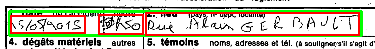
\includegraphics{ctpn_overzealous}
			\caption[\CTPN{} overzealous merging]{The \CTPN{} predicts a single box covering multiple ground truths in the same line.
			While essentially correct,
			%since a good transcription system should be able to handle this detection,
			in our measures only the largest ground truth is counted as detected.
			}
			\label{fig:ctpn_overzealous_merge}
		\end{figure}

		\begin{figure}
			\vspace{-2em}
			\begin{subfigure}{.49\linewidth}
					\caption{\FRCNN{}}\label{fig:frcnn_results}
					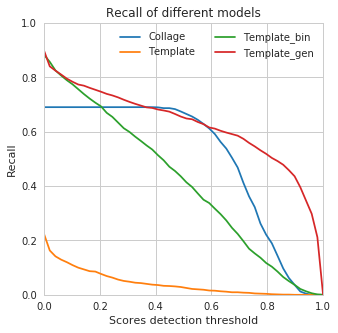
\includegraphics{frcnn_recall_scores}
					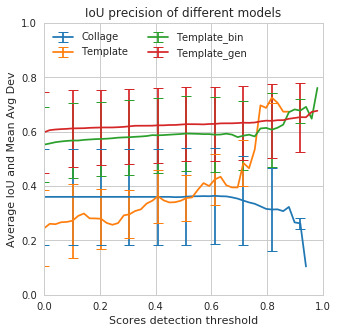
\includegraphics{frcnn_prec_scores}
					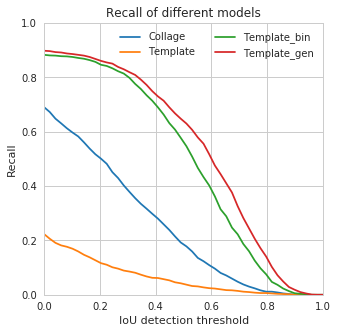
\includegraphics{frcnn_recall_iou}
			\end{subfigure}
			\rulesep
			\begin{subfigure}{.49\linewidth}
					\caption{\CTPN{}}\label{fig:ctpn_results}
					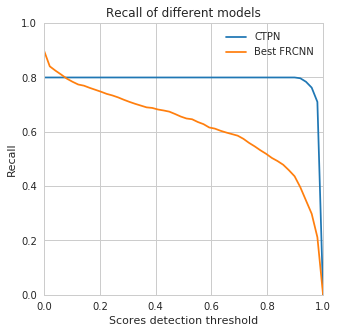
\includegraphics{ctpn_recall_scores}
					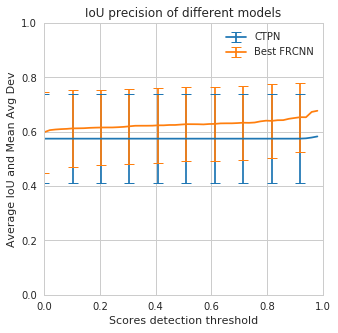
\includegraphics{ctpn_prec_scores.png}
					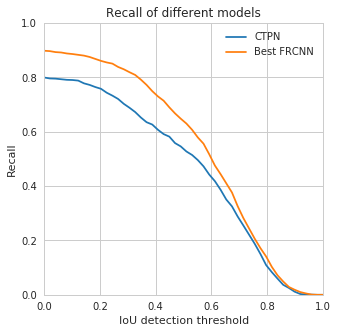
\includegraphics{ctpn_recall_iou}
			\end{subfigure}
			\caption{Text detection results}
		\end{figure}

%!TEX root = ../main.tex

\chapter{Transcription}\label{ch:transcription}

This chapter is dedicated to the problem of offine handwriting recognition, that is, given an image of a text line, find the corresponding characters and words. Although some may consider it a solved task, since many approaches achieve very good performance on a wide variety of corpora (see \autoref{sec:related_transcription}), we remind the reader that our use case poses several challenges that are not present in the controlled environments of academic contests (\autoref{sec:challenges}). Of these, we summarise the most important ones:
\begin{description}
	\item[unbefitting writing conditions] The documents are completed in a rush, soon after an accident, with no proper support structure for writting and with few format restrictions.

	\item[unconstrained recognition] Statements include text which does not admit a vocabulary for correction, such as phone numbers and license plates.

	\item[lack of annotated data] As in the case of detection, we started the project having only a database of images and no useful annotations.
\end{description}

The chapter first introduces the \CRNN{} architecture \citep{CRNN}, which has become almost a standard for optical character recognition in the recent years. Then, \autoref{sec:transcription_experiments} presents several experiments for training, including various methods of data generation. Each new experiment tries to address the weaknesses of the previous one, in a quest of reproducing the great results obtained on clean handwriting databases and in OCR. Finally, we present an overview of the obtained results in \autoref{sec:transcription_results} and why our observations prove this problem is more difficult than OCR.



%========================================================================================

\section{Convolutional Recurrent Neural Networks}\label{sec:crnn}

	%--INTRO --------------------------------------------------------------------------------

		Text transcription has preoccupied researchers for a very long time. Therefore, a large amount of ideas have been tried in order to solve this problem, of which we mention a few in \autoref{sec:related_transcription}. One of the challenges of text resides in its wide variation of appearance. For example, a free font website such as \url{www.1001fonts.com/} currently lists approximately 9500 different typefaces. Moreover, it is believed that each person has a completely unique handwriting, which is why this is still commonly used a signature. This highlights the importance of being able to represent images of text robustly, or, in other words, to extract good features that distinguish well among characters. As was previously stated, convolutional neural networks have proved very effective in this task time and again, so it is natural to use them as a first stage in a transcription architecture.

		Another peculiarity of text, which we have also mentioned in the detection chapter, is given by its sequential aspect. Few neural network architectures support arbitrarily-sized input. Of these, the recurrent neural network (RNN) has become a standard since it models well sequences of any type.

		The Convolutional Recurrent Neural Network (\CRNN{}) architecture uses the two approaches above in a unified framework to transcribe text from natural images. Considering that it achieved state-of-the-art performance in such a challenging task, we believe it is suitable for our use case as well, which is why we focused most of our efforts in this direction. Next, we detail its inner workings as they are crucial in devising our experiments.


		\begin{figure}
		\begin{subfigure}[c]{.48\linewidth}
		\begin{flushleft}
		\footnotesize
		\begin{tabular}{|l|c|}
			% \footnotesize
			\hline
			\textbf{Type} & \textbf{Configurations}						\tabularnewline	\hline
																																				\hline
			Transcription & - 																\tabularnewline	\hline
			Bi-LSTM & \#hidden units:256						\tabularnewline	\hline
			Bi-LSTM & \#hidden units:256						\tabularnewline	\hline
			Map-to-Seq & - 															\tabularnewline	\hline
			BatchNorm & - 														\tabularnewline	\hline
			Conv (7) & \#maps:512, k:$2\times2$, s:1, p:0	\tabularnewline	\hline
			MaxPool (4) & Window:$1\times2$, s:2								\tabularnewline	\hline
			Conv (6) & \#maps:512, k:$3\times3$, s:1, p:1	\tabularnewline	\hline
			BatchNorm & - 														\tabularnewline	\hline
			Conv (5) & \#maps:512, k:$3\times3$, s:1, p:1	\tabularnewline	\hline
			MaxPool (3) & Window:$1\times2$, s:2 							\tabularnewline	\hline
			Conv (4) & \#maps:256, k:$3\times3$, s:1, p:1	\tabularnewline	\hline
			BatchNorm & - 														\tabularnewline	\hline
			Conv (3) & \#maps:256, k:$3\times3$, s:1, p:1	\tabularnewline	\hline
			MaxPool (2) & Window:$2\times2$, s:2								\tabularnewline	\hline
			Conv (2) & \#maps:128, k:$3\times3$, s:1, p:1	\tabularnewline	\hline
			MaxPool (1) & Window:$2\times2$, s:2 							\tabularnewline	\hline
			Conv (1) & \#maps:64, k:$3\times3$, s:1, p:1		\tabularnewline	\hline
			Input & $W\times32$ gray-scale image 							\tabularnewline	\hline
		\end{tabular}\par
		\caption[\CRNN{} structure]{\todo{Note different from paper, use tabu, split conv part separately }}\label{fig:crnn_architecture}
		\end{flushleft}
		\end{subfigure}
		\begin{subfigure}[c]{.49\linewidth}
			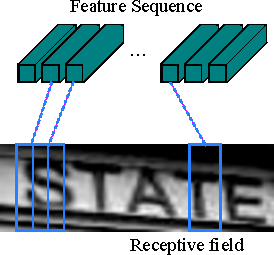
\includegraphics{crnn_rec_field}
			\caption{Image encoding into sequence of features \citep[credit to][]{CRNN}}\label{fig:crnn_sequence}
		\end{subfigure}
		\caption{The \CRNN{} architecture}
		\end{figure}

	%----------------------------------------------------------------------------------------
	\subsection{Feature extraction}
		The first part of the \CRNN{} architecture consists of a custom 7-layer CNN that transforms the input image into a sequence of high-level features. This is similar to well-known architectures, as it alternates convolutional and pooling layers (\autoref{fig:crnn_architecture}). A few particularities are important to be noted.

		First, the input is pooled differently on the vertical dimension than on the horizontal one. For the former, 4 layers with pooling windows of height 2 are used. As a result, an input of height 32 becomes a feature map of height 2. This is further reduced this to a \(\mathit{height} = 1\) feature by the last convolutional layer, which applies \(2 \times 2\) convolution with no padding. For the horizontal direction, the nework performs pooling only twice with a window of width 2. This ensures the receptive field does not become too wide and can still distinguish very narrow characters such as \{\texttt{l,i,1}\}. The network is fully convolutional, which allows inputs of any size to be processed. However, since the columns become features of the RNN, the height should be standardised. This design is well suited for images of text which are bounded vertically, but not horizontally.

		Second, the network uses batch normalisation \citep{batch_norm}, which is standard practice in recent times since it improves the performance and the stability of the network. This works by replacing the activations \(\ve{H}\) of a layer with their normalised counterparts \(\ve{H}'\), which become the new inputs for the next layer: \[
			\ve{H}' = \gamma \frac{\ve{H} - \ve{\mu}}{\ve{\sigma}} + \beta,
		\]\footnote{\todo{make miu and sigma vectors}} where \(\mu\) is a vector of means of all neurons and \(\sigma\) a vector of their standard deviations. The learnable parameters \(\gamma\) and \(\beta\) ensure the network does not lose expressive power by allowing convergence towards any mean and standard deviation. Overall, using this technique means that the composition of the batches is important, as we will see shortly.

		Finally, we use ReLU activations at each layer and bias terms for the convolution.

		%........................................................................................
		\subsubsection*{Input preprocessing}

			Input images are resized to have a heigth of 32px, while keeping their aspect ratio. As a result, their widths are different which makes it difficult to construct batch tensors. Therefore, we also define a standard input width of 250px and make sure all training images are narrower than this in the interest of avoiding horizontal deformation. Images that are shorter than the necessary width are duplicated horizontally up to this size. As opposed to padding the shorter images with blank space, this concatenation mechanism keeps a similar distribution of pixels across all batches. Note this does not produce bad training examples because we keep track of the original length when aligning the predictions and the labels.

	%----------------------------------------------------------------------------------------

	\subsection{RNN decoder}\label{sec:LSTM}
		The CNN part of the architecture encoded horizontal portions of the image (of full height) into a sequence of high dimensional features, ordered left to right (\autoref{fig:crnn_sequence}). This sequence is then consumed by an RNN decoder in order to produce character representations. To avoid the problem of vanishing gradients in long sequences, the LSTM version is employed \citep{LSTM_original} which uses a combination of gates to control the flow of information inside the cell. By default, an LSTM cell can only use past context in addition to the current input. In our case, future context can be very helpful, so a bi-directional variant of LSTM is used. 	Moreover, using a stack of two such layers allows us to capture more complex contextual dependencies.

		%........................................................................................
		\subsubsection*{Connectionist Temporal Classification}\label{sec:CTC}

			Training RNNs normally requires ground truth labels at each time step. We can see this is problematic in our context, since we only know the final sequence and not how it is aligned to the input image. Moreover, some features in the sequence can correspond to space between the characters, so there is no ground truth for them.

			This problem is solved using the Connectionist Temporal Classification method \citep[CTC; ][]{CTC}. It requires the output of the network to be a softmax output layer with \(N + 1\) units, \(N\) being the size of our alphabet \(L\). Each unit represents the probability of a symbol in the alphabet, and the extra unit corresponds to observing no label, which is denoted by ``\(-\)'', a \emph{blank} symbol . In this way, the outputs define the probabilities of all possible alignments of the input sequence with all possible output sequences.

			Additionally, the method requires a many-to-one mapping function from sequences of network outputs, denoted as \(\pi\), to actual labels, denoted as \(\bm l\): \[
				\mathcal{B}: L'^T \to L ^{\leq T},~L' = L \cup \{-\},
			\] where \(L^{\leq T}\) is the set of all possible sequences of length up to \(T\).
	 		For example, \(\mathcal{B}\) maps \mbox{$\pi$: ``\texttt{$-$fee$-$mmm$-$mm$--$ee$-$}}'' to $\bm l$:  ``\texttt{femme}'' by removing duplicates and blanks. Note that the order of these operations is important; removing blanks first results in impossibility of mapping double characters.

	 		Finally, CTC defines the probability of a given label \(\bm{l} \in L^{\leq T}\) conditioned on the input sequence \(\mathbf{x}\) as the sum of the probabilities of all output paths \(\pi\) that correspond to it:
	 		\begin{align*}
				p(\bm{l} | \bm{x}) &= \sum_{\pi:{\cal B}(\pi)=\bm{l}}p(\pi|\bm{x}), \\
				p(\pi | \bm{x}) &= \prod_{t=1}^T \bm{y}_{\pi_t}^{t},
				\label{eq:stringprob}
			\end{align*}
			where \(\bm{y}_{\pi_t}^{t}\) is the probability of observing label \(\pi_t\) at time \(t\), as outputted by the network.

			Given the exponential number of possible sequences \(\pi\) corresponding to \(\bm l\), finding the most probable label \(h(\bm{x}) = \argmax_{\bm{l} \in L^{\leq T}} p(\bm{l} | \bm{x})\) for an input \(\bm x\) becomes intractable very quickly. Therefore, an approximation is made based on the assumption that the most probable path will correspond to the most probable labelling:\[
				h(\bm{x}) \approx \mathcal{B}(\pi^*),~~ \text{where } \pi^* = \underset{\pi}{\argmax}~ p(\pi|\bm{x}).
			\] Decoding in this way can be calculated either with the backward-forward algorithm, or greedily with beam search.

			The loss function between a predicted labelling \(h(\bm{x})\) and a target ground truth label \(\bm z\) is calculated as the edit distance between the two, i.e.\ the number of insertions, deletions or substitutions needed to transform one into the other.

	%----------------------------------------------------------------------------------------

	\subsection{Training and evaluation}
		An input image flows through the convolutional layers and into the LSTM ones, whose predictions are aligned with the ground truth text as explained above. This allows the network to be trained end-to-end on pairs of images and sentences, with the error being back-propagated through all layers. In particular, the LSTM layers use Truncated Back-Propagation Through Time. Also, we noticed improvements when using dropout on the output of the final LSTM with a dropping probability \(p_\mathit{drop} = 0.2\).

		We train the network on batches of 512 images using the Adam optimiser \citep{adam} with a learning rate \(\alpha = 0.001\) and exponential decay rate for the first moment estimates \(\beta_1 = 0.5\). We also tried using an exponentially decreasing learning rate, but found it counterproductive since it needed tuning for each individual corpus or else it would slow down the learning before reaching a plateau.

		Finally, we used an alphabet of 81 characters that we identified in the corpus of the RIMES database: \(2 \times 26\) lower and upper-case letters, 10 digits, 13 French-specific letters with diacritics, and 6 symbols. In addition, we set the architecture to treat as errors differences regarding the case of letters during train time. It is important to note, though, that the distribution of characters in a corpus is not equal, as it is a feature of the language.

		%........................................................................................
		\subsubsection*{Evaluation}
			As in the case of text detection, we started with no ground truth labels on real data. Therefore, to have an objective and relevant measure of the models' performance, we also annotated the bounding boxes of the \ds{Test} dataset. However, the quality for some of these prevented us from providing an accurate transcription. Therefore, we transcribed illegible glyphs with a placeholder character that is not part of the training set. This was done so as to allow wrong predictions at this point while providing normal evaluation for the legible part.

			Given the small size of the \ds{Test} dataset of only 1400 examples, no experiments used it either for training or validation. Each model was only evaluated once on this dataset, and we recorded its performance.

			We use the \emph{normalised} character error rate (CER), and the word error rate (WER) for measuring the performance of different models, expressed as percentages: \[
			\begin{aligned}
				\cer &= \frac{100}{N} \sum_i \frac{\operatorname{dist}(\mathit{prediction}_i, \mathit{groundTruth}_i)}{\card{\mathit{groundTruth}_i}},\\
				\wer &= \frac{100}{N} \sum_i (1 - \delta (\mathit{prediction}_i, \mathit{groundTruth}_i)),
			\end{aligned}
			\]
			where the \(\operatorname{dist}()\) function evaluates the edit distance and \(\delta\) outputs 1 if its arguments are the same, letter for letter, or 0 when they differ. Note that, unless otherwise specified, we use the raw values, without discounting for placeholders in the ground truth. This results in minimally attainable error rates that are slightly above zero: \(\cer_\mathit{min} = 0.8\%,~\wer_\mathit{min} = 5.02\%\).

			Normalising the CER by the length of ground truth is important for aggregating over multiple predictions. Otherwise, mistakes in shorter words would have a heavier contribution than those in longer words. In addition, normalisation also helps in getting an intuitive understanding of the measure; for example, \CER{33} means that one character in three is wrong.

	%----------------------------------------------------------------------------------------

%========================================================================================

\section{Experiments}\label{sec:transcription_experiments}
	Considering the lack of real training data, we try to achieve our goal by the means of transfer learning: we will train our models on several different datasets and evaluate them on real data. The rest of the section presents step-by-step our experiments, describing for each of them the training data, the performance of the model and the identified weaknesses.

	%----------------------------------------------------------------------------------------

	\subsection{Academic databases}
		%........................................................................................
		\subsubsection*{Datasets}
			At the very first phase, we validated that the architecture can learn and perform handwriting recognition by training on the already-discussed RIMES database. We trained and predicted using images of single words, hence the name \ds{Word} model. This converged after seeing \(\approx 780\)k training examples to a \emph{validation} \CER{8.29},	but it did not work on our documents, where \CER{115}. We realised again the importance of pixel values, so we re-trained on \emph{binarised} words (\ds{Word_bin} model), which performed similarly on validation dataset, but had a great improvement on \ds{Test}, with \CER{61.8}. Adding dropout with probability \(p_\mathit{drop} = 0.2\) further lowers the CER by 2\% (\ds{Word_bin_drop} model).

			\begin{figure}
				
\includegraphics[width=.49\linewidth]{crnn/word_model_3}
				
\includegraphics[width=.49\linewidth]{crnn/word_model_1}
				
\includegraphics[width=.49\linewidth]{crnn/word_model_2}
				
\includegraphics[width=.49\linewidth]{crnn/word_model_4}
				\caption[Predictions of \ds{Words_bin} model]{The ground truth and the predictions are shown above the images (left and right, respectively). When there are few background elements, the prediction works reasonably well, with the exception of missing spaces.}
				\label{fig:crnn_word_drop_model}
			\end{figure}

			We note that in the examples where the model almost works (\autoref{fig:crnn_word_drop_model}) some of the errors come from the model not being able to predict spaces. This is expected since there are no examples of it in the training set, which contains only images of full words. We try to correct this by including images of multiple words and spaces. However, we cannot use full lines due to their wildly varying widths, which become a problem for making training batches. Moreover, our cutting algorithm from \autoref{sec:rimes_template} cannot always produce accurate (\texttt{image},\texttt{text}) pairs due to inconsistencies in ground truth data. Therefore, we choose to add those lines from the RIMES database which are narrower than the input width (250px). Given that there are only a few of them, approximately 1000 compared to 50\,000 words, we decide to also add similarly short lines from the IAM handwriting database \citep{iam}, which adds appoximately 2500 examples. With these, together with the words images, we train a new model (\ds{Word_short_IAM}) which again achieves a similarly good performance on its validation dataset. Surprisingly though, it performs much worse on the statements, with a \CER{104}. We believe this is due to the additional English corpus from the IAM database which confuses the language model of the LSTM.

		%........................................................................................
		\subsubsection*{Outcome}
			The experiments on academic corpora revealed several key differences between them and the target dataset. One consists of the influence of pixel values (gray vs binary) and of background elements (\autoref{fig:crnn_dashes}), which increases validation CER from 17\% to 37\%. Another is given by the style of the handwriting: the one in RIMES database is mostly cursive, whereas IAM and the statements have more ``printscript'' style (using block letters). Then, the content is important too: we observe a consistent difference between strict and lowercase-only matching (\autoref{tab:transcription_academic}), meaning the model has trouble differentiating the case of words. Finally, we observe the great importance of the language model. Besides the problems introduced by using an English corpus, the continuous, gramatically-correct sentences in the RIMES database precondition the LSTM in a way that does not apply to the statements, whose fields are mostly names, addresses and numbers.

			In general, we validated through many small experiments that it is possible to learn to transcribe handwriting from our corpus by training on a different one. While the results so far are cannot be used in practice, the performance improvements demonstrate that transfer learning is a valid strategy, so we continue to explore it. In addition, we validate the results of \citet{MDLSTM_dropout}, showing that dropout consistently improves the performance. Therefore, all further models will use it, with \(p_\mathit{drop} = 0.2\).

			\begin{figure}
				
\includegraphics[width=.32\linewidth]{crnn/short_ok_1}
				
\includegraphics[width=.32\linewidth]{crnn/short_ok_2}
				
\includegraphics[width=.32\linewidth]{crnn/short_ok_3}
				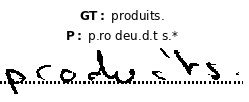
\includegraphics[width=.32\linewidth]{crnn/short_dash_1}
				
\includegraphics[width=.32\linewidth]{crnn/short_dash_2}
				
\includegraphics[width=.32\linewidth]{crnn/short_dash_3}
				\caption[Influence of backgrond elements]{The same model \ds{Word_bin_drop} was evaluated on clean images from RIMES (top) and their variants with added indicator line (bottom). This simple perturbation increases the error rate by \(20\%\). }
				\label{fig:crnn_dashes}
			\end{figure}

			\begin{table}
				\centering
				\begin{tabular}{| l | *{4}{c |}}\hline
					\textbf{Dataset name} & \textbf{CER strict} & \textbf{CER lower} & \textbf{CER ascii} & \textbf{WER}\\\hline
					\ds{Word} & 115.52 & 109.98 & 109.83 & 98.28\\
					\ds{Word_bin} & 62.43 & 59.44 & 59.43 & 94.25\\
					\ds{Word_bin_drop} & 60.58 & 57.71 & 57.71 & 94.83\\
					\ds{Word_short_IAM} & 104.19 & 100.24 & 100.15 & 98.78\\
					% \ds{Word_short} & 103.70 & 100.97 & 100.74 & 98.71\\
					\ds{Word_short_drop} & 103.77 & 100.36 & 100.17 & 97.70\\\hline
				\end{tabular}
				\caption[Academic datasets results]{Results of the \CRNN{} model trained on different datasets from the academic databases RIMES and IAM. Largely impractical, but useful to confirm the influence of various factors.}\label{tab:transcription_academic}
			\end{table}

	%----------------------------------------------------------------------------------------

	\subsection{Generator}\label{sec:generator}

		%... Description ........................................................................
			Inspired by the state-of-the-art achievements in OCR with synthetic data \citep{synthetic_data}, we try to address the limitations of the academic databases using a similar approach. Specifically, we adapt the code released by aforementioned authors to better suit our task by bringing the following improvements:
			\begin{description}
				\item[jiggle letters] Humans rarely have pixel-accurate alignment of their handwriting; likewise for the horizontal distribution of letters. Therefore, we randomly jiggle letters side-ways as well as up and down.

				\item[rotate, do not bend] As we noticed in the RIMES database, the baseline of handwriting is sometimes skewed from the horizontal. However, it is rarely bent. We reflect this in the generated text.

				\item[size and binarisation] Allow the generation of binarised text of specified height so as to avoid later resizing and its artefacts.

				\item[document-like noise] Add salt and pepper noise similar to that produced by optical scanners. Also add background elements such as randomly dashed indicator lines on text's baseline position.

				\item[real corpora and format] Generate real text based on publicly available datasets of person names, street and city names. Also generate according to various standard formats for dates, phone numbers and license plates.

				\item[cursive rendering] Allow rendering of fonts with ligatures to better resemble cursive handwriting.
			\end{description}

			\begin{figure}
				\setkeys{Gin}{height=16pt}
				\setkeys{Gin}{width=.5\ginnatwidth}
				% \setkeys{Gin}{width=.32\linewidth}
				
\includegraphics[width=6cm]{crnn/generated/987}\hspace{3mm}
				
\includegraphics{crnn/generated/3}\hspace{3mm}
				
\includegraphics{crnn/generated/12}\\\vspace{3mm}
				
\includegraphics{crnn/generated/27}\hspace{3mm}
				
\includegraphics{crnn/generated/35}\hspace{3mm}
				
\includegraphics{crnn/generated/47}\\\vspace{3mm}
				
\includegraphics{crnn/generated/57}\hspace{3mm}
				
\includegraphics{crnn/generated/65}\hspace{3mm}
				
\includegraphics{crnn/generated/83}
				\caption[Generated images]{Examples of text generated by our tool. Dates, license plates and numbers are generated randomly according to different formats, whereas the others are sampled from various corpora. Names are not real, but randomly matchd between common first and last names.}
				\label{fig:generated_images}
			\end{figure}

		%........................................................................................
		\subsubsection*{Datasets}
			Equipped with the powerful tool above, we generate a corpus of size similar to RIMES (50\,000 training examples, \ds{Gen_50k}) using a selection of 25 handwriting-style fonts (examples in \autoref{fig:generated_images}). This converged to a validation \CER{4.6} after seeing, interestingly, the same amount of training examples as RIMES-trained model (\(\approx 750\)k). We noticed that further training for about twice as long brings improvements to the validation word error rate (\(\approx -3.5\%\)) while the CER remains constant. This suggests that the LSTM picks up further subtleties in the language model. However, the results on \ds{Test} were slightly worse that previous best, at \CER{67.31}. Evaluating this model on RIMES data exposes a key observation: it does not generalise there, either, having \CER{75.8}. While we actually wanted this data to be different, we expected it to be an extension to RIMES dataset. Seeing it is not, we trained a model on both of them (\ds{Gen_50K_RIM}) which achieved a new low, with \CER{45.78}.

			\urldef{\vLetter}\url{https://www.vletter.com/help/about-vletter.html}
			We hypothesised that the sub-par performance of the generated data was due to the small variation of fonts compared to human handwriting. Therefore, we created a database of 900 cursive fonts, each being a customised version of a real person's handwriting\footnote{\vLetter}; 100 of them were kept for validation. The model trained on this, \ds{Gen_800f} is better than the initial one of generated-only data (\ds{Gen_50k}). However, it still does not caputre all natural features of handwriting, performing slightly worse than \ds{Gen_50k_RIM}. Increasing the dataset size to 1 million examples (\ds{Gen_1M}) further approaches the mixed data model. Surprisingly, doubling the input resolution proves counterproductive (\ds{Gen_1M_64}).

		%........................................................................................
		\subsubsection*{Outcome}
			\begin{table}
				\centering
				\begin{tabular}{| l | *{4}{c |}}\hline
					\textbf{Dataset name} & \textbf{CER strict} & \textbf{CER lower} & \textbf{CER ascii} & \textbf{WER}\\\hline
					\ds{Gen_50k} & 67.31 & 63.67 & 63.44 & 93.82\\
					\ds{Gen_50k_RIM} & 45.78 & 42.06 & 42.13 & 85.78\\
					\ds{Gen_800f} & 49.02 & 43.98 & 43.66 & 86.21\\
					\ds{Gen_1M} & 46.06 & 39.85 & 39.55 & 83.62\\
					\ds{Gen_1M_64} & 50.24 & 43.29 & 42.97 & 85.06\\\hline
					(Best RIMES) & 60.58 & 57.71 & 57.71 & 94.83\\\hline
				\end{tabular}
				\caption[Generated datasets results]{Performance of models trained on different versions of generated datasets.}
				\label{tab:transcription_generated}
			\end{table}

			\begin{figure}
				\setkeys{Gin}{width=.3\linewidth}
				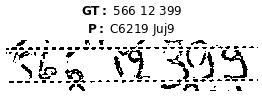
\includegraphics[valign=c]{crnn/gen_model_2}\hspace{5mm}
				\includegraphics[valign=c]{crnn/gen_model_1}\hspace{5mm}
				\includegraphics[valign=c]{crnn/gen_model_3}
				\caption[Understandably wrong predictions (1)]{A model trained on \ds{Gen_1M} makes wrong predictions on \ds{Test} dataset. However, examining them character by character, we realise they are not so off from what is shown in the image. For example, in the middle image the ``\texttt{0}'' is taken for an ``\texttt{O}'', the ``\texttt{1}'' really resembles ``\texttt{A}'', ``\texttt{/}'' character does look like a slanted ``\texttt{1}'' and the final ``\texttt{13}'' is undistinguishable from ``\texttt{B}''.
				}\label{fig:transcription_wrong}
			\end{figure}

			The series of experiments proved it is possible to learn relevant handwriting features and compensate for a small and uniform dataset (\autoref{tab:transcription_generated}).  However, significantly more data is needed to cover for the differences between natural and synthetic handwriting, in our case by a factor of 20. A mixed dataset seems to cover the best of both worlds, achieving the best performane at \CER{45.78}.

			Given that the results are still of no practical use, we inspected in more detail the generated data and the models' predictions. Looking at some examples in \autoref{fig:transcription_wrong}, we see that individual glyphs in the image actually correspond well to what the model predicts. The problem is that we, as humans, choose to interpret the whole differently than the concatenation of its parts. At the same time, parts derive their meaning from that of the whole. For example, glyphs that look like slanted bars are considered ones when grouped with another digit, but slashes when separating groups of digits, since we assume that the latter represents a date.

	%----------------------------------------------------------------------------------------

	\subsection{Corpus type}

		%... Description ........................................................................
			\urldef{\ICDAR}\url{http://u-pat.org/ICDAR2017/program_competitions.php}
			Based on the above observations, we try to address the shortcomings of the architecture. Specifically, we believe the LSTM language model suffers from the wild differences in the format of data, e.g.\ dates versus names. To the best of our knowledge, no good results have been published on such highly heterogeneous data. For example, the old problem of MNIST handwriting recognition is only concerned with digits, possibly arranged into strings. Additionally, the documents in ICDAR handwriting recognition competitions\footnote{\ICDAR} contain text from archaic documents which presents complex glyphs but still use normal language. Therefore, we try to split the challenge into smaller, more homogeneous sub-problems. However, instead of doing this manually, we will only provide information about the type of corpus that a given text belongs to and let the architecture learn and switch between different formats.

			To accomplish the above, we group the data into logical corpora which represent their type, or context. For the final pipeline, we envision that the assignment of text to a given corpus happens at detection time, where its location on the page can provide strong hints in this regard. Therefore, the categories are as follows:
			\begin{description}
				\item[Person names\vspace{-1.5em}]

				\item[Numbers] These are mostly phone numbers, but include, in general, any string of digits. We note that in real data some of these can also contain one or two characters, as they represent the contract ID.

				\item[Dates] These can come under a variety of formats, such as \texttt{27/04/03} and \texttt{22 Mar 2013}, with many possible delimiters. We group them all into the same category.

				\item[Hours] Similarly to dates, there are many possible formats for these as well.

				\item[Addresses] An address usually comprises of several parts: number, street, post code and city. In the statements, these are usually split in groups of two, over two lines. As such, address format usually follows a strict rule: ``\texttt{<digits>, <letters and spaces>}''.

				\item[License plates] These come in two formats which, unfortunately, are very different from one another: the new one is ``\texttt{AA 111 AA}'', while the old one is ``\texttt{1111 AAA 11}''.

				\item[Observations] This can include any natural language observations, makes and models of cars, country names, etc.
			\end{description}
			Although the formats are still not completely separated, most of them are well defined and have to be chosen from a smaller pool.

		%........................................................................................
		\subsubsection*{Strategy 1: preconditioning the LSTM}
			A body of work that is similar to our task was done in the area of image captioning. Most architectures there are also made up from a CNN feature extractor and an RNN language model, but the exact implementation details can have large influences on the result. For a first trial, we follow the implementation of \citet{lstm_precondition}, who precondition the LSTM by setting its hidden state to an encoding of the last convolutional feature map. Then they input and predict word vectors.

			We use a similar approach for providing the corpus information alongside the image features. We encode corpus class into an indicator vector \(\mathbbm{1}(c = 1) \in \{0, 1\}^F\), where \(F\) is the LSTM input size and \(c\) the unique integer ID of the corpus\footnote{This encoding scheme is also known as \emph{one-hot} encoding, in a vector of size \(F\)}. We use this as the first item in the features sequence, thus providing the same hidden state initialisation for all images belonging to the same corpus.

			We generate a new dataset as above, this time also keeping its origin information as corpus ID. A model trained on this, \ds{Gen_corpus_pre}, comes close to previous best, at \CER{47.94}. However, it does not improve on it. We believe there are two reasons behind this: first, the corpus feature vector is mostly filled with zeros when projected in image space, since there are just 7 different corpora and \(F = 512\) image features; second, our sequences are two to three times longer than those in image captioning, and not even the LSTM architecture can keep context for so long.

		%........................................................................................
		\subsubsection*{Strategy 2: add extra features}
			To overcome the problem of a very long sequence, we add the corpus information as extra features to the LSTM input, at all time steps. This is encoded as before, in an indicator vector \(\mathbbm{1}(c = 1) \in \{0,1\}^7\) (now only of necessary width), and is concatenated to the image features \(\mathcal{F}_t\) of each time step in the sequence\footnote{\todo{Use concatenation operator}}:\[
				\mathcal{F}'_t = \mathcal{F}_t \circ \mathbbm{1}(c = 1).
			\]

			Since the previous dataset already contains corpus information, we reuse it for training a new model with this configuration, \ds{Gen_corpus_all}. It achieves a new best, at \CER{41.76}. We observe it correctly learns formats of corpora, such as always predicting long numbers in groups of two digits, despite the ground truth being without white space.


		%........................................................................................
		\subsubsection*{Outcome}
			\begin{table}
				\centering
				\begin{tabular}{| l | *{4}{c |}}\hline
					\textbf{Dataset name} & \textbf{CER strict} & \textbf{CER lower} & \textbf{CER ascii} & \textbf{WER}\\\hline
					\ds{Gen_corpus_pre} & 47.94 & 40.75 & 40.44 & 81.82\\
					\ds{Gen_corpus_all} & 41.76 & 37.03 & 36.70 & 81.11\\\hline
					(Best generated) & 46.06 & 39.85 & 39.55 & 83.62\\\hline
				\end{tabular}
				\caption[Corpora information results]{Performance of a \CRNN{} model trained on a generated dataset of 1 million examples which include information about corpus of origin.}\label{tab:transcription_corpus}
			\end{table}

			Our hypothesis about the heterogeneity of data was validated and we sucessfully decrease it by bringing extra information into the architecture. However, the exact implementation makes a big difference, since the sequences we feed into the LSTM can be very long.

			\begin{figure}
				\begin{subfigure}[b]{.3\linewidth}
					\includegraphics{crnn/cor_model_2}
					\caption{}\label{fig:cor_model_2}
				\end{subfigure}
				\begin{subfigure}[b]{.3\linewidth}
					\includegraphics{crnn/cor_model_1}
					\caption{}\label{fig:cor_model_1}
				\end{subfigure}
				\begin{subfigure}[b]{.3\linewidth}
					\includegraphics{crnn/cor_model_3}
					\caption{}\label{fig:cor_model_3}
				\end{subfigure}
				\caption[Understandably wrong predictions (2)]{A model trained with knowledge about the type of text it sees understands better the format of different strings, e.g.\ in \subref{fig:cor_model_3} it completes the second dot by itself. However, it still strugles to make sensible choices, like in the case of \subref{fig:cor_model_2}. There, the second digit coult be taken for a ``\texttt{6}'', if it were on its own; but seeing the first glyph is an actual ``\texttt{6}'' gives us an indication that the second cannot be the same thing.}\label{fig:corpus_wrong}
			\end{figure}
			We again inspect in detail the type of mistakes that the model is making (\autoref{fig:corpus_wrong}) and observe that these are mostly related to the path that the model finds through the activations matrix. Specifically, the approximation in \autoref{sec:CTC} makes it predict the character of maximum activation. For example, for the last digit in \autoref{fig:cor_model_3} is an unusual ``\texttt{2}'' that \emph{does} have a part looking like a regular ``\texttt{9}''; this part probably overlaps maximally with the model's representation of ``\texttt{9}'' and that is what the model predicts.

	%----------------------------------------------------------------------------------------

	\subsection{Elastic deformations}
		%... Description ........................................................................
			Despite using over 800 realistic handwriting fonts for generating data, and affine transformations on top such as slanting and skewing, we observed even the best models still do not capture all the variation in natural handwriting. This pointed us to the advice of \citet{elastic_distortions}, who describe a method of data augmentation for handwritten digits. Specifically, they propose using random displacement fields \(\Delta \ve{x}, \Delta \ve{y} \in \operatorname{rand}(-1,1)\) which correspond to uncontrolled oscillations of the hand muscles, dampened by inertia. These are then used as parameters of an interpolation for sampling in the original image. However, using the purely random values results in a noisy distortion of the image. This can be accommodated by first convolving the fields \(\Delta \ve{x}, \Delta \ve{y}\) with a Gaussian kernel of standard deviation \(\sigma\), which becomes the elastic coefficient. Seeing that small values of sigma produce too much deviation (\autoref{fig:elastic_4}), we select sigma from a normal distribution \(\mathcal{N}(8, 2)\), but threshold it at values bigger than 5. Another important parameter is \(\alpha\) which controls the displacement amount. While the authors recommend a hard value of \(\alpha=34\), we found this to be dependent on the image size. Therefore, we empirically determined a good relation to be \(\alpha = 1.5 \times H\), where \(H\) is the height of the image.
			\begin{figure}
				\begin{subfigure}[t]{.32\linewidth}
					\includegraphics{crnn/elastic}
					\caption{Original image}\label{fig:elastic_0}
				\end{subfigure}
				\begin{subfigure}[t]{.32\linewidth}
					\includegraphics{crnn/elastic4}
					\caption{\(\sigma = 4\)}\label{fig:elastic_4}
				\end{subfigure}
				\begin{subfigure}[t]{.32\linewidth}
					\includegraphics{crnn/elastic8}
					\caption{\(\sigma = 8\)}\label{fig:elastic_8}
				\end{subfigure}
				\caption[Elastic deformations]{Examples of influence of the elastic coefficient \(\sigma\)}
			\end{figure}

		%........................................................................................
		\subsubsection*{Datasets and outcome}
			We enhanced the generator from \autoref{sec:generator} to include this type of deformations as well, and, as before, we produced a dataset of 1 million examples, with corpus information included, \ds{Gen_elastic}. We observed from the start a much better performance on the validation dataset, compared to the previous best model, \ds{Gen_corpus_all} (\autoref{fig:elastic_cer_drop}). However, this does not readily transfer to the \ds{Test} dataset, as it attains a \mbox{\CER{42.2}} that is close to the one before. Moreover, we let this model train for much longer than any previous ones and observe that although its \emph{validation} performance remains stable, at a given point it starts to perform worse on \ds{Test}(\autoref{tab:elastic_corpus}). It is important to note that this type of overfit cannot be detected during training since we do not validate on \ds{Test}. Therefore, the model is picking up very subtle features which differentiate generated data from real one, although for us both look the same.

			\begin{figure}
				\includegraphics{crnn/elastic_drop}
				\caption[Improvements of elastic deformations]{The curves show the training evolution of validation CER and accuracy \mbox{(\(= 1 - \wer\))} of the best models with (blue) and without (orange) elastic deformations.}\label{fig:elastic_cer_drop}
			\end{figure}

			\begin{table}
				\centering
				\begin{tabular}{| l | *{5}{c |}}\hline
					\textbf{Dataset name} & \textbf{epochs} & \textbf{CER strict} & \textbf{CER lower} & \textbf{CER ascii} & \textbf{WER}\\\hline
					\ds{Gen_elastic_1}    &  8 & 45.14 & 38.59 & 38.30 & 83.33\\
					\ds{Gen_elastic_2}    & 18 & 43.97 & 38.95 & 38.70 & 82.90\\
					\ds{Gen_elastic_3}    & 31 & 42.20 & 36.92 & 36.64 & 81.68\\
					\ds{Gen_elastic_4}    & 48 & 45.29 & 40.16 & 39.89 & 83.41\\\hline
					(Best ``with-corpus'')& 31 & 41.76 & 37.03 & 36.70 & 81.11\\\hline
				\end{tabular}
				\caption[Elastic deformation results]{Performances obtained when training on a corpus with elastic deformations included, at different training times.
				}\label{tab:elastic_corpus}
			\end{table}


%========================================================================================

\section{Results}\label{sec:transcription_results}
	\begin{table}
		\centering
		\begin{tabular}{| l | *{4}{c |}}\hline
			\textbf{Dataset name} & \textbf{CER strict} & \textbf{CER lower} & \textbf{CER ascii} & \textbf{WER}\\
			\hline
			\ds{Word} & 115.52 & 109.98 & 109.83 & 98.28\\
			\ds{Word_bin} & 62.43 & 59.44 & 59.43 &\bf 94.25\\
			\ds{Word_bin_drop} &\bf 60.58 &\bf 57.71 &\bf 57.71 & 94.83\\
			\ds{Word_short_IAM} & 104.19 & 100.24 & 100.15 & 98.78\\
			% \ds{Word_short} & 103.70 & 100.97 & 100.74 & 98.71\\
			\ds{Word_short_drop} & 103.77 & 100.36 & 100.17 & 97.70\\
			\hline

			\ds{Gen_50k} & 67.31 & 63.67 & 63.44 & 93.82\\
			\ds{Gen_50k_RIM} & 45.78 & 42.06 & 42.13 & 85.78\\
			\ds{Gen_800f} & 49.02 & 43.98 & 43.66 & 86.21\\
			\ds{Gen_1M} &\bf 46.06 &\bf 39.85 &\bf 39.55 &\bf 83.62\\
			\ds{Gen_1M_64} & 50.24 & 43.29 & 42.97 & 85.06\\
			\hline

			\ds{Gen_corpus_pre} & 47.94 & 40.75 & 40.44 & 81.82\\
			\rowcolor{LightGreen}
			\ds{Gen_corpus_all} &\bf 41.76 &\bf 37.03 &\bf 36.70 &\bf 81.11\\
			\hline

			\ds{Gen_elastic_1} & 45.14 & 38.59 & 38.30 & 83.33\\
			\ds{Gen_elastic_2} & 43.97 & 38.95 & 38.70 & 82.90\\
			\ds{Gen_elastic_3} &\bf 42.20 &\bf 36.92 &\bf 36.64 &\bf 81.68\\
			\ds{Gen_elastic_4} & 45.29 & 40.16 & 39.89 & 83.41\\
			\hline\hline
			\ds{Test \footnotesize{(600 examples)}} & 21.59 & -- & -- & 62.11\\
			\hline
		\end{tabular}
		\caption[All transcription results]{Performances of different models. \textbf{Bold} entries are the best in their category, while the \colorbox{LightGreen}{highlighted} entry is the best overall.
		}\label{tab:transcription_results}
	\end{table}


	% corpus_all and elastic_3 are very close for lower

	We summarise the results of our experiments in \autoref{tab:transcription_results}. We see that large amounts of generated data overcome the limitations of a uniform dataset such as RIMES and that adding contextual information such as corpus type helps the architecture build better language models. However, the generated data does not bring benefits as big as it does in OCR and printed text recognition. We believe this is expected due to a number of reasons. First, printed text is usually put on a hard support; therefore all images of such text represent just an affine transformation of the original. This is in contrast to handwritten text which presents many subtle variations at stroke level. Then, text-in-the-wild usually comprises of words and language; with a little effort we can generate all such possible instances. In contrast, our task has to cope with almost infinite combinations of digits and letters. Finally, fonts used for printed text have unambiguous glyphs, in general; apart from \{\texttt{i,1,l}\}, all glyphs are intentionally very different from one another. However, in handwritting, the same glyph can correspond to different characters and only context can solve the ambiguity.

	We also observe that the architecture overfits to generated data, despite the large number of fonts and the elastic deformations. This, again, makes the task easier for printed text, since virtually all of it was generated by an existing font, unlike handwriting which is almost unique to every person.

	Finally, we tried to explore the maximum capabilities of the current transcription system by fine-tuning the best model on a subset of \ds{Test} dataset. Using 800 text examples for training and 600 for testing, we managed to improve the performance up to \mbox{\CER{21}}, \WER{62}. Unfortunately, we do not have a human level error rate to compare with. Also, it is unclear whether more training data would be beneficial or a more powerful architecture is needed for further improvements.



\bibliography{refs}             % this causes the references to be listed
\bibliographystyle{plainnat}       % see natbib for other possible values

% \include{chapters/appendix}

\end{document}
